\documentclass[12pt,a4paper,twoside,openright]{book}
%\usepackage[work]{MCthesis}			% you can select this to work




\usepackage[final]{MCthesis}				% this is for the final submission


%%%%%%%%%%%%%%%%%%%%%%%%%%%%%%%%%%%%%%%%%%%%%%%%%%%%%%
%%%%%%%%%%%%%%%%%%%%%%%%%%%%%%%%%%%%%%%%%%%%%%%%%%%%%%
\usepackage[utf8]{inputenc} 		% allow utf-8 input
\usepackage[T1]{fontenc}    		% use 8-bit T1 fonts
\usepackage{lmodern}
\usepackage[hidelinks]{hyperref}           			% simple URL typesetting
\usepackage{booktabs}       		% professional-quality tables
\usepackage{nicefrac}       		% compact symbols for 1/2, etc.
\usepackage{microtype}      		% microtypography
\usepackage{xcolor}         			% colors
\usepackage{amssymb,amsmath,amsfonts,amsbsy, amsthm}
\usepackage{bm}             			% bold vectors
\usepackage{listings} 			% to include R-Code
\usepackage[section]{placeins}		% forces floats to appear in the section they are placed in
\usepackage{listings} 			% to include R-Code
\usepackage[nosectionbib]{apacite}	% bibliography example
\usepackage[toc,page]{appendix}
\usepackage{framed}
\usepackage{listings}
\usepackage{float}
\usepackage{xcolor}
\usepackage{soul}
\usepackage{bbm}
\usepackage{tikz}
\usepackage{pdflscape}
\usepackage{subcaption}
\usepackage{booktabs}
\usepackage{comment}
\usepackage{siunitx} % optional, but nice for numbers

\usepackage{tabularx}
\usepackage{array}
\usepackage{threeparttable}

\newtheorem{proposition}{Proposition}
\newtheorem{lemma}{Lemma}
\newtheorem{theorem}{Theorem}

%\sethlcolor{red}
%%%%%%%%%%%%%%%%%%%%%%%%%%%%%%%%%%%%%%%%%%%%%%%%%%%%%%
%%%%%%%%%%%%%%%%%%%%%%%%%%%%%%%%%%%%%%%%%%%%%%%%%%%%%%
\usepackage{blindtext}
%%%%%%%%%%%%%%%%%%%%%%%%%%%%%%%%%%%%%%%%%%%%%%%%%%%%%%
\usepackage{etoolbox}   % for \ifstrempty
\usepackage[nameinlink,noabbrev]{cleveref} % optional, for \cref

\usepackage{titlesec}

% Numbered chapters: 6 Discussion
\titleformat{\chapter}[hang]
  {\normalfont\Huge\bfseries}
  {\thechapter}{1em}{}

% Unnumbered chapters: Discussion
\titleformat{name=\chapter,numberless}[hang]
  {\normalfont\Huge\bfseries}
  {}{0pt}{}

% Spacing: left, before, after
\titlespacing*{\chapter}{0pt}{0pt}{2em}


% --- Theorem style: "Assumption C1. (Consistency.)"
\newtheoremstyle{assumpstyle}%
  {3pt}{3pt}% space above/below
  {}% body font
  {}% indent
  {\bfseries}% head font
  {}% punctuation after head
  {.5em}% space after head
  {%
    \thmname{#1}\thmnumber{ #2}.%
    \ifstrempty{#3}{}{ \textit{(#3).}}%
  }%

\theoremstyle{assumpstyle}

% --- Common identification assumptions: C-I1, C-I2, ...
\newtheorem{idassumpC}{Assumption}
\renewcommand{\theidassumpC}{C-I\arabic{idassumpC}}

\newtheorem{modassumpC}{Assumption}
\renewcommand{\themodassumpC}{C-M\arabic{modassumpC}}

% --- FE-specific identification assumptions: FE-I1, FE-I2, ...
\newtheorem{idassumpFE}{Assumption}
\renewcommand{\theidassumpFE}{FE-I\arabic{idassumpFE}}

% --- SeqGPLVM-specific identification assumptions: SG-I1, SG-I2, ...
\newtheorem{idassumpSG}{Assumption}
\renewcommand{\theidassumpSG}{SG-I\arabic{idassumpSG}}

% --- FE-specific modeling assumptions: FE-M1, FE-M2, ...
\newtheorem{modassumpFE}{Assumption}
\renewcommand{\themodassumpFE}{FE-M\arabic{modassumpFE}}

% --- SeqGPLVM-specific modeling assumptions: SG-M1, SG-M2, ...
\newtheorem{modassumpSG}{Assumption}
\renewcommand{\themodassumpSG}{SG-M\arabic{modassumpSG}}


% --- Make cleveref print "Assumption C1" etc.
\crefname{idassumpC}{Assumption}{Assumptions}
\crefname{modassumpC}{Assumption}{Assumptions}
\crefname{idassumpFE}{Assumption}{Assumptions}
\crefname{idassumpSG}{Assumption}{Assumptions}
\crefname{modassumpFE}{Assumption}{Assumptions}
\crefname{modassumpSG}{Assumption}{Assumptions}

%%%%%%%%%%%%%%%%%%%%%%%%%%%%%%%%%%%%%%%%%%%%%%%%%%%%
% SET VARIABLES FOR TITLE PAGE
\title{A Comparative Study of Two Methods for Estimating Causal Effects with Time-Varying Treatments under Time-Invariant Unmeasured Confounding}
\author{Ali Setareh Kokab}
\fromCity{Tübingen}
\matnr{6332297}
\date{\today} % submission date



%%%%%%%%%%%%%%%%%%%%%%%%%%%%%%%%%%%%%%%%%%%%%%%%%%%%
% SET VARIABLES FOR  SUPERVISION AND EXAMINERS
\supervisor{Prof. Dr. Holger Brandt}{}{}
\reviewer{Prof. Dr. Augustin Kelava}{}{}


%%%%%%%%%%%%%%%%%%%%%%%%%%%%%%%%%%%%%%%%%%%%%%%%%%%%%%%%%%%%%%%%%%%




\begin{document}
\maketitle
% % % % % % % % % % % % % % % % % % % % % % % % % % % % % % % % % % % % % % % % % % % % % % % % 

\input{sections/introduction}
\chapter{Background and related work}
\label{chap:literature_review}

Methods for longitudinal causal inference can be organized along two main dimensions: 
the structure of the causal diagram and the causal target of interest. 
The structure of the causal setting is typically represented by a directed acyclic graph (DAG) 
that encodes the assumptions about the data generating process and the causal relationships 
between the variables \cite{pearlCausalityModelsReasoning2009}. The presence or absence of 
treatment-confounder feedback 
and unobserved confounders are important features of the causal structure that can affect the 
choice of estimation method. The causal target of interest, on the other hand, is driven by the 
research question and scientific context of the study \cite{lundbergWhatYourEstimand2021}. Different methods may be designed to estimate 
different causal targets, such as the average treatment effect at a specific time point, the cumulative 
effect of treatment over time, or the contrast between two specific treatment regime. Having these 
two dimensions in mind, in the 
following sections, we will review the relevant literature on longitudinal causal inference 
and the methods exist to address confounding.

\section{Potential outcomes and treatment regimes}
The causal targets are often formalized in the potential-outcomes framework \cite{rubinEstimatingCausalEffects1974}. 
In this framework, we define the potential outcome of individual $i$ as $Y_i(a)$, representing the outcome that would be observed if 
the treatment $A$ were set to a specific value $a$. Note the difference between the observed outcome $Y_i$ and the 
potential outcome $Y_i(a)$ which is an unobserved variable, 
as we can only observe the outcome under the treatment that was actually assigned to. Similarly, in the longitudinal setting, we can define the potential outcome at time $t$ for a 
static\footnote{The static here is to contrast with a 
dynamic treatment regime, where treatments depends on the values of the confounders \cite{moodieDemystifyingOptimalDynamic2007}. In this thesis we only consider static treatment regimes.} treatment regime 
$\bar{a}_t = (a_0, a_1, a_2, \ldots, a_t)$ as $Y_{i,t+1}(\bar{a}_t)$, 
representing the outcome that would be observed if the treatment were set to specific values at each 
time point. In a similar way, the 
potential value of confounders at time $t$ can also be defined as $X_{i,t}(\bar{a}_{t-1})$, 
representing the value of the confounder at time $t$ that would be observed if the treatment 
were set to specific values at each time point up to $t-1$\footnote{Here we follow the Robins indexing convention to emphasize the temporal ordering of the treatments, 
confounders and (repeated) outcome \cite{hernanCausalInferenceWhat2023}. Counfounders at time time $t$ is measured after the treatment at time $t-1$ 
and before the treatment at time $t$. Moreover, the potential outcome is indexed at time $t+1$ to reflect 
the fact that the outcome is determined after the treatment while the measured outcome at time $t$ may act 
as a confounder for the treatment at time $t$ and the outcomes at later time points.}.

\section{Treatment-confounder feedback}
Treatment-confounder feedback occurs when the treatment at time $t$ can affect the confounders at later 
time points. This creates a feedback loop between the treatment and the confounders, 
which can lead to bias if not properly adjusted for. in Figure \ref{fig:sample_dags} (b), these feedback loops 
are represented by the purple arrows from $A_t$ to subsequent $X_{t+k}$ where $1 \le k \le T-k$. These structures 
are problematic for standard regression-based methods, as they can lead to collider 
bias if we condition on the confounders at time $t$; And the confounder 
\section{Identification under sequential ignorability}
There are well-established methods for 
identifying and estimating the average potential outcomes of statatic treatment regimes when treatment-confounder feedback is present.
These methods—known as the g-methods—include the g-formula \cite{robinsEstimationCausalEffects2008,snowdenImplementationGComputationSimulated2011}, marginal structural models (MSMs) \cite{robinsMarginalStructuralModels2000}, 
and structural nested models (SNMs) \cite{vansteelandtStructuralNestedModels2014}. 
They all rely on the assumption of sequential ignorability, 
which states that the potential outcomes 
\section{Treatment-confounder feedback}
\begin{comment}  
Longitudinal causal inference is a broad area of research with a rich literature. There are 
two main dimensions along which the longitudinal causal estimators can be organized. The first is the structure 
of the causal setting, typically represented by a directed acyclic graph (DAG) 
with a set of nodes $\mathbf{V}$ and a set of directed edges $\mathbf{E}$. 
Each node in the graph represents a variable and each directed edge 
represents a causal relationship between two variables. 
The structure of the causal diagram encodes the assumptions about the 
data generating process and the causal relationships between the variables \cite{pearlCausalityModelsReasoning2009}. This includes 
features such as the presence or absence of treatment-confounder feedback or presence 
of unobserved confounders as shown in Figure \ref{fig:sample_dags}. Some methods are designed to work in specific types 
of causal structures, while others are more general and can be applied to a wider range of settings.


The second dimension is about the causal target of interest, that is, the 
estimand addressed by the method. This dimension is driven by the research question and 
the scientific context of the study \cite{lundbergWhatYourEstimand2021}. 
For example, in a longitudinal study with time-varying treatments, 
one might be interested in estimating the average treatment effect at a specific time point, 
the cumulative effect of the treatment over time, or the effect of a specific treatment regime. A particular method 
might be able to estimate one or more of these targets, but not all of them.


\section{Setup and causal estimands in longitudinal studies}
\subsection{Potential outcomes under static and dynamic treatment regimes}
The causal targets are often formalized in the potential-outcomes framework \cite{rubinEstimatingCausalEffects1974}. 
In this framework, we define the potential outcome of individual $i$ as $Y_i(a)$, representing the outcome that would be observed if 
the treatment $A$ were set to a specific value $a$. Then one common causal target, the average treatment effect (ATE), is defined as 
the difference in expected potential outcomes under different treatment values, i.e., $\text{ATE} = \mathbb{E}[Y_i(1) - Y_i(0)]$ 
for a binary treatment. Note the difference between the observed outcome $Y_i$ and the 
potential outcome $Y_i(a)$ which is an unobserved variable, 
as we can only observe the outcome under the treatment that was actually assigned to.

Similarly, in the longitudinal setting, we can define the potential outcome at time $t$ for a 
\emph{static} treatment regime 
$\bar{a}_t = (a_1, a_2, \ldots, a_t)$ as $Y_{i,t+1}(\bar{a}_t)$, 
representing the outcome that would be observed if the treatment were set to specific values at each 
time point. In a similar way, the 
potential value of confounders at time $t$ can also be defined as $X_{i,t}(\bar{a}_{t-1})$, 
representing the value of the confounder at time $t$ that would be observed if the treatment 
were set to specific values at each time point up to $t-1$. The static here is to contrast with a 
\emph{dynamic} treatment regime, where treatments depends on the values of the confounders \cite{moodieDemystifyingOptimalDynamic2007}. 

\subsection{Treatment-confounder feedback and temporal ordering}

Here we follow the Robins style of indexing convention to emphasize the temporal ordering of the treatments, 
confounders and (repeated) outcome \cite{hernanCausalInferenceWhat2023}. Counfounders at time time $t$ is measured after the treatment at time $t-1$ 
and before the treatment at time $t$. Moreover, the potential outcome is indexed at time $t+1$ to reflect 
the fact that the outcome is determined after the treatment while the measured outcome at time $t$ may act 
as a confounder for the treatment at time $t$ and the outcomes at later time points. 
\end{comment}

\section{Identification under sequential ignorability}
When all confounders are measured, there are well-established methods for 
identifying and estimating causal effects in longitudinal settings. 
These methods include g-methods such as the g-formula \cite{robinsEstimationCausalEffects2008}, marginal structural models (MSMs) \cite{robinsMarginalStructuralModels2000}, and structural nested models (SNMs) \cite{vansteelandtStructuralNestedModels2014}. 
These methods rely on the assumption of sequential ignorability, 
which states that there are no unmeasured confounders at each time point.

methods to deal with unmeasured confounding can be divided based on how they 
deal with the sequential ignorability assumption. some methods such as the deconfounder 
methods try to retain the sequential ignorability assumption by estimating a substitute 
for the unmeasured confounders, 
while FE-MSM assume a version of sequential ignorability that is conditional on the unit-specific unobserved heterogeneity component, 
while other methods such as instrumental variable methods or proxy variable methods try to relax the 
sequential ignorability assumption by using additional data with a specific structure.

\subsection{G-methods}
\cite{vansteelandtStructuralNestedModels2014}
\cite{robinsEstimationCausalEffects2008}
\cite{keilParametricGformulaTimetoevent2014}

\subsubsection{Marginal structural models}
\cite{robinsMarginalStructuralModels2000}
\cite{neugebauerCausalInferenceLongitudinal2007}


\section{Methods for unmeasured confounding in longitudinal settings}
\subsection{Time-invariant unmeasured confounding and panel structure}
\cite{imaiWhenShouldWe2019} -> \cite{blackwellEffectPoliticalAdvertising2024} 

\subsection{Latent-variable approaches}
\cite{wangBlessingsMultipleCauses2019}
\cite{bicaTimeSeriesDeconfounder2020}
\cite{hattSequentialDeconfoundingCausal2024}

\subsection{Proximal causal inference}
\cite{tchetgenIntroductionProximalCausal2020} -> \cite{yingProximalCausalInference2023}, \cite{deanerProxyControlsPanel2023}


\subsection{Instrumental-variable approaches for longitudinal unmeasured confounding}
\cite{angristIdentificationCausalEffects1996} -> \cite{michaelInstrumentalVariableEstimation2020} ->\cite{chengInstrumentalVariableEstimation2024}





There are different causal targets that can be defined in the longitudinal setting. A  
 such as the average treatment effect at time $t$, the cumulative effect of the treatment over time, or the effect of a specific treatment regime. The choice of the causal target depends on the research question and the scientific context of the study. For example, if we are interested in the effect of a treatment at a specific time point, we might focus on estimating the average treatment effect at that time point. If we are interested in the overall effect of a treatment over time, we might focus on estimating the cumulative effect of the treatment. If we are interested in the effect of a specific treatment regime, we might focus on estimating the effect of that regime compared to another regime.
This inde that the potential outcome is defined at time $t+1$ 
to emphasize that the outcome is determined after the treatment at time $t$, where the treatment at time $t$ can affect the confounders at later time points.
The average treatment effect at time $t$ can then be defined as $\text{ATE}_t = \mathbb{E}[Y_{i,t+1}(\bar{a}_t) - Y_{i,t+1}(\bar{a}'_t)]$ for two different treatment regimes $\bar{a}_t$ and $\bar{a}'_t$.
as $Y_i(a_1, a_2, \ldots, a_t)$, representing the outcome that would be observed if the treatment were set to specific values at each time point. The average treatment effect at time $t$ can then be defined as $\text{ATE}_t = \mathbb{E}[Y_i(a_1, a_2, \ldots, a_t) - Y_i(a'_1, a'_2, \ldots, a'_t)]$ for two different treatment regimes.




\begin{figure}[htbp]
\centering

\begin{subfigure}{0.8\textwidth}
\centering
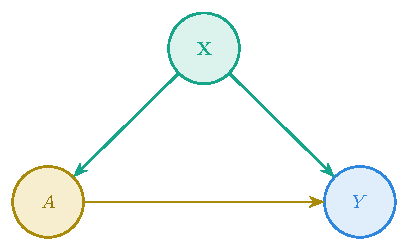
\includegraphics[width=\linewidth]{figures/build/simple_dag.pdf}
\caption{A simple causal DAG with treatment $A$, outcome $Y$, and confounder $X$. The confounder $X$ is a common cause of both the treatment $A$ and the outcome $Y$, which can lead to confounding bias if not properly adjusted for.}
\end{subfigure}

\vspace{0.6cm}

\begin{subfigure}{0.8\textwidth}
\centering
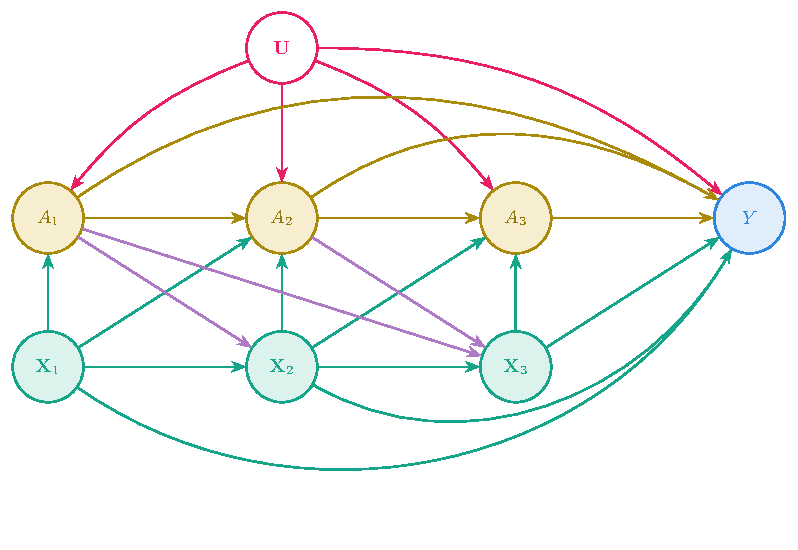
\includegraphics[width=\linewidth]{figures/build/treatment_covariate_feedback.pdf}
\caption{A longitudinal causal DAG with time-varying treatments $A_t$, time-varying confounders $X_t$, and an unobserved confounder $U$.
Filled nodes represent observed variables, while the unfilled node represents an unobserved variable. Arrows 
from $A_t$ to $X_{t+1}$ represent treatment-confounder feedback, where the treatment at time $t$ can affect the confounders at later time points.}
\end{subfigure}

\caption{Two examples of causal DAGs. The first DAG (a) represents a simple static setting with a single treatment and outcome, while the second DAG (b) represents a more complex longitudinal setting with time-varying treatments.}
\label{fig:sample_dags}
\end{figure}

 

and the second dimension is the presence or absence of such feedbacks.
To situate the two methods that we are going to compare in this thesis, we will review 
There are different suggested identification strategies for specifically designed to address such feedbacks such as the g-formula or inverse probability of treatment weighting (IPTW) \cite{robinsEstimationCausalEffects2008a}. 
However, these identification strategies rely on the assumption of 
sequential ignorability, which states that the researcher 
has gathered all the \emph{required} data for the causal analysis or more  
formally there are no unmeasured confounders between the treatments and the outcome at each time point. %In the most general case, 
%confounders can be seen as a common cause of two or more variables in the causal graph. 
%In the context of longitudinal data, we are often concerned about unmeasured confounders effecting the 
%treatment assignment and the outcome at each time point.  
This is a strong assumption and often violated in real world settings. 

To address the problem of unmeasured confoundedness in static settings, there have been 
different methods proposed. Some need additional data with a very specific 
structure such as instrumental variable methods \cite{angristIdentificationLocalAverage1996} 
or using proxy variables \cite{tchetgenIntroductionProximalCausal2020}, 

while others rely on strong assumptions about the data generating process such as the deconfounder method \cite{wangBlessingsMultipleCauses2019}.
\chapter{Methods}
\label{chap:method}
\section{Notation and setup}
\label{sec:notation}
In this section we introduce the notation and the setup used throughout this thesis. 
Let $i=1, \ldots, N$ index the individuals in the study and let $t=0, \ldots, T$ 
index the time points at which measurements are taken. We denote the treatment 
variable at time $t$ for individual $i$ as $A_{it}$, which can take on values from a 
predefined set of treatment options. In this thesis, 
we assume a binary treatment, $A_{it} \in \{0,1\}$. We adopt the convention that treatment 
is absent at the beginning of the study, $t=0$ and therefore $A_{i0} = 0$ 
for all individuals $i$. 
The outcome variable at 
time $t$ for individual $i$ is 
denoted as $Y_{i,t+1}$ to emphasize that the outcome is measured after the treatment at time $t$.
We also consider a set of observed covariates $X_{it}$, 
which may include both time-varying 
and time-invariant variables. The history of treatment and covariates up to time $t$ for 
individual $i$ is represented as
$\bar{A}_{it} = (A_{i1}, A_{i2}, \ldots, A_{it})$ and $\bar{X}_{it} = (X_{i1}, X_{i2}, \ldots, X_{it})$, 
respectively. We denote the potential outcome at time $t$ for individual $i$ under a specific treatment
regime $\bar{a}_t = (a_1, a_2, \ldots, a_t)$ as $Y_{i,t+1}(\bar{a}_t)$. Finally, we use $U_i$ 
to represent \emph{structural} unmeasured confounders that are time-invariant for individual $i$. 

We also define truncated versions of the treatment and covariate histories from \(k\) 
steps prior up to time \(t\) as \(\underbar{A}_{i,t-k}\) and \(\underbar{X}_{i,t-k}\), respectively. 
The outcome setup we are focusing on is a single outcome measured at the end of 
the study, i.e., at time T+1, denoted as $Y_{i,T+1}$. This is the setup considered in
\cite{blackwellEffectPoliticalAdvertising2024} and it is a special case of the setup in
\cite{hattSequentialDeconfoundingCausal2024} who consider outcomes measured at each time point. This 
choice is both motivated by the specific application they consider 
(political advertising) and technical reasons related to the consistency of the IPTW-FE estimator.

Moreover, since the asymptotic properties and consistency of the IPTW-FE estimator relies on the 
truncated potnetial outcomes, we can define the truncated potential outcomes as
$Y_{i,T+1}(\underline{a}_{T-k}) \equiv Y_{i,T+1}(\overline{A}_{i,T-k-1},\, \underline{a}_{i,T-k})$. This 
definition represents the potential outcome of manipulating 
the last $k$ treatment values, while leaving the earlier treatment values as observed. In this way, 
the earlier treatments before the last $k$ time points can be thought of as part of the baseline covariates. 
In this section, we describe the two proposed methods 
for adjusting for unmeasured time-invariant confounding: the fixed-effect marginal 
structural model (FE-MSM) proposed by \citeA{blackwellEffectPoliticalAdvertising2024}
and the sequential Gaussian process latent variable model (SeqGPLVM) 
proposed by \citeA{hattSequentialDeconfoundingCausal2024} when it is used 
in conjunction with IPTW estimation of MSM. We first describe the common set of
assumptions required by of these methods, and then go 
into the details of the steps of each method. The causal target of interest for both methods 
is the average truncated potential outcome.  

FE-MSM consists of two stages: (i) a treatment model that 
estimates the propensity scores, conditioning on both observed 
covariates and individual fixed effects that capture the unmeasured time-invariant confounding, 
and (ii) a marginal structural model that uses the estimated propensity scores in stage one to adjust for confounding using IPTW.

SeqGPLVM in combination with MSM on the other hand, consists of three stages: 
(i) a latent variable model (SeqGPLVM) that estimates a substitute 
for the unmeasured confounder based on the observed treatment sequence, (ii) estimating 
the propensity scores using a treatment model that conditions on both observed 
covariates and the estimated unmeasured confounder substitute, and (iii) 
a marginal structural model that uses the estimated propensity scores in stage two 
to adjust for confounding using IPTW. It is worth mentioning that SeqGPLM can be used with any
other estimation methods as well, such as g-computation or doubly robust methods, 
but we focus on IPTW estimation of MSM for comparability with FE-MSM.

\section{Common assumptions}
\label{sec:assumptions}
The common assumptions for both FE-MSM and SeqGPLVM-MSM are stated below. 
The assumptions can be categorized into two groups: identification assumptions and 
modeling assumptions. Identification assumptions, 
are the assumptions which are needed to write target causal estimands such as 
$\mathbb{E}[Y_i(\underline{\mathbf{a}}_{T-k})]$ in terms of observed data. 
Based on the identification strategy and the estimator of choice, 
certain quantities must be modeled. 
For example, estimating a marginal structural model for the target causal estimand using 
inverse probability of treatment weighting (IPTW) requires modeling the 
propensity scores. Modeling assumptions are about the 
requirements placed on these models in order to have unbiased or consistent estimates. 
Throughout the text, 
we use C, I, and M to denote common, identification, and modeling 
assumptions, respectively.
% --- Common assumptions (C1, C2, ...) ---
% Assumes you already defined the assumpC environment (C-prefix) in the preamble.

\begin{idassumpC}[Consistency]\label{ass:C-consistency}
The observed outcome for each individual under their observed treatment history equals
the potential outcome under that treatment history. Formally, if $\bar{A}_{iT}=\bar{\mathbf{a}}_{iT}$, 
then $Y_{i}=Y_{i}(\bar{\mathbf{a}}_{iT})$. 
Moreover, $Y_{i} = Y_{i}(\underline{\mathbf{a}}_{i,T-k})$ if 
$\bar{\mathbf{A}}_{iT}=\left(\bar{\mathbf{A}}_{i,T-k-1},\underline{\mathbf{a}}_{i,T-k}\right)$.
\end{idassumpC}

\begin{comment}

\begin{assumpC}[Positivity]\label{ass:C-positivity}
\[
\Pr\!\left[ A_t = a_t \,\middle|\, 
\bar{A}_{t-1} = \bar{a}_{t-1},\,
\bar{X}_t = \bar{x}_t \right] > 0
\]

for all values $(\bar{a}_{t-1}, \bar{x}_t)$ with

\[
\Pr\!\left[ \bar{A}_{t-1} = \bar{a}_{t-1},\,
\bar{X}_t = \bar{x}_t \right] \neq 0
\]

in the population of interest, and for all $a_t \in \mathcal{A}_t$.
\end{assumpC}

\end{comment}

\begin{idassumpC}[No interference]\label{ass:C-no-interference}
The treatment assignment for one individual does not affect the potential outcomes of
other individuals. This assumption is also known as the no spillover assumption.
\end{idassumpC}

\begin{idassumpC}[Time-invariance of unmeasured confounding]\label{ass:C-timeinvariant-uc}
The unmeasured confounding is assumed to be
time-invariant. That is, $\mathbf{U}_{i,t} = \mathbf{U}_i$ for $t \in \{1,\dots,T\}$. We can then write 
conditional ignorability as 
\[
\{ Y_{i,t+1}(\bar{\mathbf{a}}_{t}),\, \bar{\mathbf{X}}_{i,t+1}(\bar{\mathbf{a}}_{t}) \}
\perp\!\!\!\perp
A_{it}
\mid
\bar{\mathbf{X}}_{it},\,
\bar{\mathbf{A}}_{i,t-1} = \bar{\mathbf{a}}_{t-1},\,
\mathbf{U}_i .
\]
Note that this assumption is about the true underlying data-generating process and cannot be  
used for identification directly since $\mathbf{U}_i$ is unmeasured. 
\end{idassumpC}

\begin{idassumpC}[Positivity]\label{ass:C-positivity}
For all treatment times $t = T - k + 1, \ldots, T$, 
and all histories $(\bar{\mathbf{X}}_t, \bar{\mathbf{A}}_{t-1}, \boldsymbol{\eta}_i)$ 
with positive probability, every treatment level has positive probability:
\[
\mathbb{P}(A_t = a_t \mid \bar{\mathbf{X}}_t = \bar{\mathbf{x}}_t,\ \bar{\mathbf{A}}_{t-1} = 
\bar{\mathbf{a}}_{t-1}, \boldsymbol{\eta}_i) > 0 \quad \text{for all } a_t \in \mathcal{A}_t
\]
Where $\boldsymbol{\eta}_i$ represents the unit-specific fixed effect in the FE-MSM model 
or the confounder substitute in the SeqGPLVM model. This assumption  particularly
is necessary for the identification of $\mathbb{E}[Y_i(\underline{\mathbf{a}}_{T-k})]$.
\end{idassumpC}



\input{sections/method/first_stage.tex}
\input{sections/method/outcome.tex}
\section{Comparison of FE-MSM and SeqGPLVM}
\label{sec:comparison}
\paragraph{FE-MSM}
The Fixed-Effects MSM (FE-MSM) addresses time-invariant unmeasured confounding by incorporating unit-specific fixed effects directly into the propensity score model.

Unit-Specific Sequential Ignorability: This method relies on the assumption that treatment is randomized conditional on the observed history and a time-constant unit-specific effect $\alpha_i$.
Estimation Procedure: We obtain estimates for the propensity parameters $\beta$ and the unit effects $\alpha_i$ via **Conditional Maximum Likelihood**. This approach is justified under **large-$N$, large-$T$ asymptotics, where the bias from noisy fixed-effect estimation (the incidental parameters problem) fades over time.
Weighted Least Squares: Once the fixed-effect weights are constructed, the MSM parameters $\gamma$ are estimated by solving a weighted estimating equation, which reduces to **Weighted Least Squares (WLS)** for our linear specification. We use a **robust (sandwich) variance estimator** to obtain valid Wald confidence intervals.

\paragraph{SeqGPLVM}

In contrast to the point-estimate approach of FE-MSM, the SeqGPLVM captures unmeasured confounding by inferring a posterior distribution $q(Z)$ over a latent substitute $Z_i$.

Handling Circular Dependency: To avoid the "circular dependency" created by using $Z_i$ as a covariate in a separate propensity model, we use the estimated propensities from the SeqGPLVM **directly** to build the IPTW weights.
Multiple Imputation (MI)-Style Procedure: To propagate the latent uncertainty from the GP-based treatment model, we draw $S$ samples $Z^{(s)} \sim q(Z)$. For each draw, we:
    1.  Compute draw-specific propensities and weights $W^{(s)}$.
    2.  Fit the weighted MSM to obtain a draw-specific estimate $\hat{\gamma}^{(s)}$ and robust covariance $V^{(s)}$.
Rubin’s Rules for Pooling: The final point estimate is the average across draws, $\bar{\gamma} = S^{-1}\sum \hat{\gamma}^{(s)}$. The total variance is calculated using **Rubin’s within/between decomposition**, $T = W + (1 + 1/S)B$, which explicitly accounts for the variability induced by the uncertainty in the inferred latent confounder.



Although the seqgplvm can be used in the settings in which the outcome is observed at every time point, 
since the asymptotic properties and consistency of their IPTW-FE estimator 
relies on having less number of N than T (assumption )
Based on the consistency assumption \ref{ass:C-consistency}, we can define 
truncated potential outcomes 

\begin{comment}

\begin{figure}[ht]
\centering
\resizebox{\textwidth}{!}{
\begin{tikzpicture}[
    font=\small,
    % ADD THIS LINE:
    ampersand replacement=\&, 
    arr/.style={-Latex, thick},
    box/.style={
        draw, rounded corners, align=left,
        inner xsep=5mm, inner ysep=3.5mm,
        text width=0.42\linewidth % Changed from 0.44 to 0.42
    },
    header/.style={
        draw, rounded corners, align=center,
        inner xsep=5mm, inner ysep=2.5mm,
        text width=0.42\linewidth, % Changed from 0.44 to 0.42
        font=\bfseries
    },
    stage/.style={
        font=\bfseries,
        align=right,
        text width=0.20\linewidth, % Increased width
        anchor=east                % Added to fix alignment
    },
    midnote/.style={
        draw, rounded corners, fill=gray!10,
        align=center, inner xsep=2.5mm, inner ysep=2.5mm,
        text width=0.16\linewidth
    }
]

% --- Matrix: All '&' replaced with '\&' ---
\matrix (m) [
    matrix of nodes,
    nodes in empty cells,
    row sep=10mm,
    column sep=12mm,
    nodes={box, anchor=north}
] {
    |[header]| FE--MSM \& |[header]| SeqGPLVM \\
    {\textbf{MSM / estimand.}\\
    Choose $k$ and specify an MSM for $Y_i(d_{T-k:T})$.}
    \&
    {\textbf{MSM / estimand.}\\
    Choose $k$ and specify an MSM for $Y_i(d_{T-k:T})$.}\\
    {\begin{minipage}[t]{\linewidth}
        \begin{enumerate}\setlength\itemsep{1pt}\setlength\parskip{0pt}
        \item No interference
        \item Consistency
        \item Positivity
        \item \textbf{Unit-specific ignorability}
        \item \textbf{Truncated Marginal Structural Model}
        \end{enumerate}
    \end{minipage}}
    \&
    {\begin{minipage}[t]{\linewidth}
        \begin{enumerate}\setlength\itemsep{1pt}\setlength\parskip{0pt}
        \item No interference
        \item Consistency
        \item Positivity
        \item \textbf{Time-invariant unmeasured confounding}
        \item \textbf{Conditional Markov model}
        \item 
        \end{enumerate}
    \end{minipage}}\\
    {\textbf{Identification.}\\
    Given (claimed) ignorability, causal effects can be estimated\\
    by MSM/IPTW using propensities conditional on $(X, A, Z)$.}
    \&
    {\textbf{Identification.}\\
    Given (claimed) ignorability, causal effects can be estimated\\
    by MSM/IPTW using propensities conditional on $(X, A, Z)$. } \\
    {\textbf{Propensity estimation.}\\
    Specify and estimate $\pi_{it}(x_t, d_{t-1}; \beta, \alpha_i)$\\
    (FE MLE). }
    \&
    {\textbf{Stage 1: SeqGPLVM.}\\
    Fit GP+CMM latent factor model to infer $Z_i$ and/or compute\\
    $\hat{\pi}_{it}=\hat{p}(A_{it}\mid A_{i,t-1},X_{it},Z_i)$. } \\
    {\textbf{Construct weights.}\\
    IPTW / stabilized weights from $\hat{\pi}_{it}$\\
    (trim if needed). }
    \&
    {\textbf{Construct weights (this thesis).}\\
    Use $\hat{\pi}_{it}$ from SeqGPLVM directly to build IPTW weights.\\
    \emph{(Original: plug $\hat{Z}_i$ into an outcome model.)} } \\
    {\textbf{Outcome stage.}\\
    Fit MSM by weighted regression / estimating equations. }
    \&
    {\textbf{Outcome stage.}\\
    Fit MSM by weighted regression / estimating equations. } \\
};

% --- Row labels ---
\node[stage] at ($(m-2-1.west)+(-12mm,0)$) {Target};
\node[stage] at ($(m-3-1.west)+(-12mm,0)$) {Identification assumptions};
\node[stage] at ($(m-4-1.west)+(-12mm,0)$) {Estimation assumptions};
\node[stage] at ($(m-5-1.west)+(-12mm,0)$) {Treatment\\ model};
\node[stage] at ($(m-6-1.west)+(-12mm,0)$) {Weights};
\node[stage] at ($(m-7-1.west)+(-12mm,0)$) {Outcome};

% --- Vertical arrows ---
\foreach \r/\rp in {2/3,3/4,4/5,5/6,6/7} {
    \draw[arr] (m-\r-1.south) -- (m-\rp-1.north);
    \draw[arr] (m-\r-2.south) -- (m-\rp-2.north);
}

% --- Central "common output" callout ---
%\node[midnote] (pi) at ($(m-5-1.east)!0.5!(m-5-2.west)$) {Outputs\\$\hat{\pi}_{it}$};
%\draw[arr] (m-5-1.east) -- (pi.west);
%\draw[arr] (m-5-2.west) -- (pi.east);

\end{tikzpicture}
}
\caption{Stage-aligned comparison of FE--MSM and SeqGPLVM. The pipelines differ in how propensities are estimated (fixed effects vs. latent factor + GP), but both feed into IPTW and a weighted MSM fit.}
\label{fig:flow_compare_rows_clean}
\end{figure}
\end{comment}


\chapter{Simulation study}
\label{chap:simulation_study} 
\section{Data generating process}
To evaluate the finte sample performance of the two proposed method, 
we conduct a simulation study based on the DGP taken 
from Section 5.1 of \citeA{blackwellEffectPoliticalAdvertising2024}. 
In this 
DGP, the scenario which we simulate is a study design 
where individuals are exposed to a binary treatment
(e.g., receiving a political advertisement) over a period 
fixed period of time, and the outcome of interest
is measured only once at the end of the study period 
(e.g., voting behavior). The treatment assignment
is influenced by both observed covariates and an 
unmeasured time-invariant confounder (e.g., political
leaning). The outcome is affected by the treatment 
received at the final time point, the cumulative 
effect of treatments received in the last three time points, 
the mean of observed covariates over time, 
and the unmeasured confounder. 

We simulate longitudinal data for 
$n \in \{200, 500, 1000\}$ individuals. For the
length of the time serieses for each n, we consider 
three different lenghts: $\rho = n/T$ 
with $\rho \in \{5,10,50\}$. The data is balanced,
menaning that each individual has 
the same number of time points. 
In Eq.~\eqref{eq:blackwell_scm}, we present 
the structural causal equations for the DGP. 
Here, $\operatorname{expit}(x) = \frac{1}{1 + e^{-x}}$ and 
$\bar{X}_{iT} = \frac{1}{T}\sum_{t=1}^T X_{it}$.

\begin{subequations}\label{eq:blackwell_scm}
\begin{align}
U_i &:= \varepsilon_i,
\qquad
\varepsilon_i \sim \operatorname{Unif}(-a,a).
\\
X_{it} &:= -\frac{1}{2}\mathbbm{1} + \varepsilon_{it},
\qquad
\varepsilon_{it} \sim \mathcal{N}(0,\Sigma).
\\
A_{it} &:= \mathbbm{1}\!\left\{\eta_{it} \le
\operatorname{expit}\!\left(U_i+\varphi A_{i,t-1}+\beta^\top X_{it}\right)\right\},
\qquad \eta_{it} \sim \operatorname{Unif}(0,1)
\\
Y_{iT} &:= U_i + \tau_F A_{iT} + \tau_C \sum_{t=T-3}^{T-1} A_{it}
+ \gamma^\top \bar X_{iT} + \epsilon_{iT},
\qquad \epsilon_{iT} \sim \mathcal{N}(0,1)
\label{eq:blackwell_scm_outcome}
\end{align}
\end{subequations}

We simulate for two different values of $a \in \{1, 2\}$ \hl{to control the
contribution of the unmeasured confounder $U_i$ to the variance of the linear predictor.} 
We simulate for two different number of covariates $p \in \{2, 4\}$ 
to see the effect of the dimensionality 
of covariates. 
The coefficients are set to $\beta = (-0.5, -0.5)^{\top}$ when $p=2$ and 
$\beta = (-0.5, -0.5, 1, -0.5)^{\top}$ when $p=4$. \hl{(add some note about why we chose 
these coeffs based on the variance or sth)}. We set $\varphi = 0.3$. %Note that we generate 
The covariates $X_{it}$ are generated exogenously to 
the treatments solely for the sake of simplicity where  $\Sigma_{jj} = 1$ and $\Sigma_{jj'} = 0.2$ for $j \neq j'$. By doing this, the ground truth 
values for the causal targets of interests conincide wit the DGP parameters. 
%So we do not have the 
%treatment-confounder feedback. This is done to isolate the effect of
%adjusting for unmeasred time-invariant confounding and make the simulation simpler and it has important 
%implications in interpreting the causal effects. see section \ref{estimation}. 
Also note that theere is no dynamics 
in the covariates and the distribution of $X_{it}$ is the same for all time points. The parameters 
for the outcome model are set to $\tau_F = 1$, $\tau_C = 0.3$, and $\gamma = (1, 0.5)^{\top}$ 
when $p=2$ and when $p=4$, $\gamma = (1, 0.5, 1, 1)^{\top}$. The causal DAG for 
the DGP is shown in Figure~\ref{fig:dgp-dag}. 
\ref{fig:dgp-dag}.
\begin{figure}[ht]
    \centering
    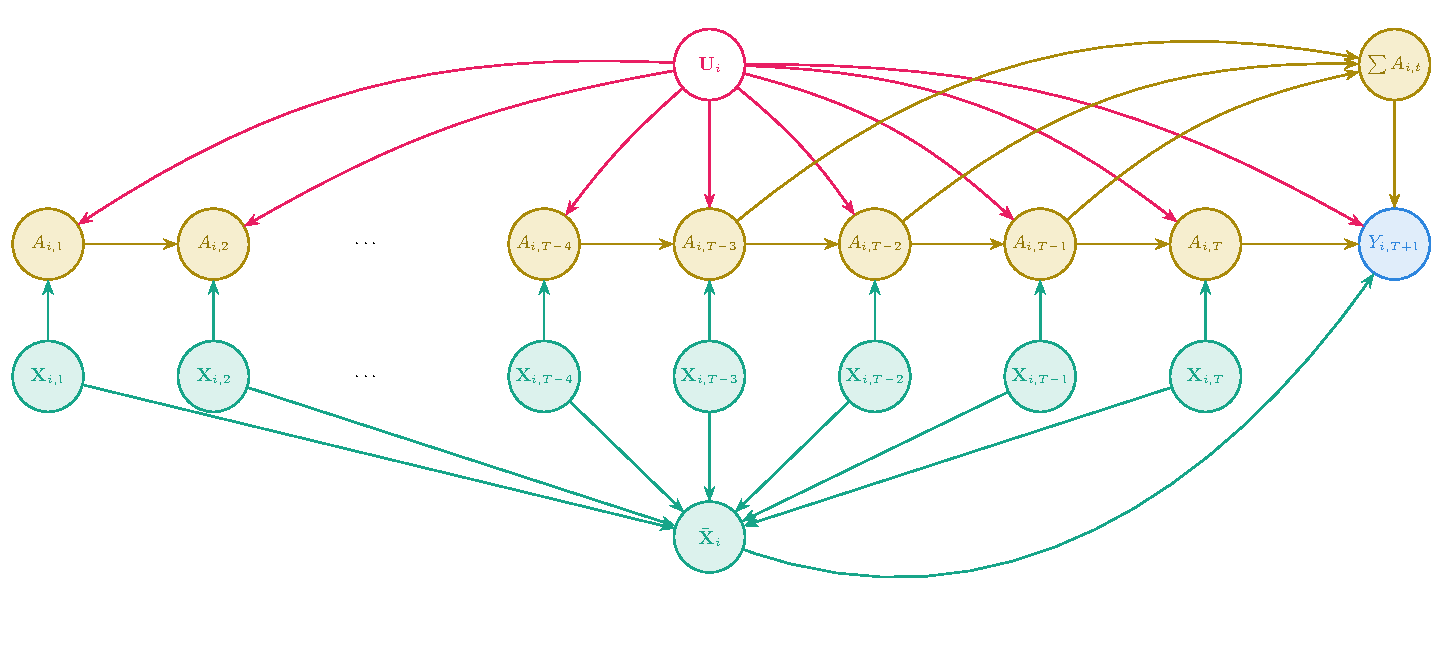
\includegraphics[width=\textwidth]{figures/build/dgp_dag.pdf}
    \caption{Data generating process causal DAG.}
    \label{fig:dgp-dag}
\end{figure}

\section{Estimation}
\label{estimation}
For defining our causal targets, first we need to specify the 
causal questions of interest. 
Define 
$$S_K(\underbar{a}_{T-K}) := \sum_{t=T-K}^{T-1} a_t 
\in \{0,1,2,\dots, K\}$$ 
as the sum 
of treatments received in the last $K$ time points before $T$, where $K+1$ 
represents the intervention window.  In real world applications, 
the choice of $K$ is based on the research question and the domain 
knowledge about the relevant time window for the treatment effects. 
In this simulation, we set $K=3$ to match the dependence structure of the 
outcome on the treatments in the DGP.

We are interested in two causal questions.
What is the average effect of the treatment received at the 
final time on the 
final outcome while holding fixed the sum of the earlier 
treatments within the intervention window, marginlized over the natural 
values of the treatments this treatment window? 
Mathematically, 
this is defined as
$\mathbb{E}\left[ Y_{iT}\left(a_T = 1, S_3 = s)\right) 
- Y_{iT}\left(a_T = 0, S_3 = s\right) \right]$. 
The second causal question is: what is the
average effect of receiving one additional treatment in 
the last three time points, 
before $T$ on the final outcome while keeping the final treatment 
fixed, marginalized over the natural 
values of the treatments in this window? To express 
this mathematically, we can write it as
$\mathbb{E}\left[Y_{iT}\left({S_3 = s, 
A_{iT} = a}\right) - Y_{iT}\left({S_3 = s+1, 
A_{iT} = a}\right)\right]$. 

To answer both of these causal questions, a marginal structural 
model is proposed  
that relates the assigned treatments to the expected potential 
outcome at the final time: 
$\mathbb{E\left[Y_{iT}\left(\underbar{a}_{T-k}\right)\right]} = 
g(\underbar{a}_{T-k}, \gamma_0)$, where 
$g(\underbar{a}_{T-k}, \gamma_0)$ is the true unkown function 
parameterized by $\gamma_0$. Our job is 
to first propose a function $f(\underbar{a}_{T-k}, \gamma)$ 
and then estimate its parameters $\gamma$. In this 
DGP, the ground truth function $g$, is: 
\begin{equation}
    \label{eq:truemsm}
    g\left(\underline{a}_{T-k}; \gamma_0 \right) = \alpha_0 + \tau_{F} a_T + \tau_{C} \sum_{t=T-3}^{T-1} a_t
\end{equation}

to see this, we begin from Eq.~\eqref{eq:blackwell_scm_outcome}. First note that since this is 
a sctructural equation model, we can replace the random variables 
by their interventional values. So we have:
\[
Y_{iT}\!\left(\underbar{a}_{T-k}\right)
= U_i + \tau_F a_T + \tau_C \sum_{t=T-3}^{T-1} a_t + \gamma^\top \bar X_{iT}(\underbar{a}_{T-k}) + \epsilon_{iT}.
\]
Taking the expectation on both sides and making use of 
the exogeneity of the covariates and treatments, we have:
\begin{align}
\label{eq:truemsmproof}
\mathbb{E}\!\left[Y_{iT}\!\left(\underbar{a}_{T-k}\right)\right]
&= \mathbb{E}[U_i] + \tau_F a_T + \tau_C \sum_{t=T-3}^{T-1} a_t
   + \gamma^\top \mathbb{E}[\bar X_{iT}] + \mathbb{E}[\epsilon_{iT}] \\
&= \mathbb{E}\!\left[U_i + \gamma^\top \bar X_{iT}\right]
   + \tau_F a_T + \tau_C \sum_{t=T-3}^{T-1} a_t \\
&= \alpha_0 + \tau_F a_T + \tau_C \sum_{t=T-3}^{T-1} a_t,
\qquad
\alpha_0 := \mathbb{E}\!\left[U_i + \gamma^\top \bar X_{iT}\right]
\end{align}
 
From Eq.~\eqref{eq:truemsm}, it can be seen: 

\begin{align*}
        &\mathbb{E}\left[ Y_{iT}\left(a_T = 1, S_3 = s\right) - Y_{iT}\left(a_T = 0, S_3 = s\right) \right] = \tau_F\\
        &\mathbb{E}\left[ Y_{iT}\left(a_T = a, S_3 = s+1\right) - Y_{iT}\left(a_T = a, S_3 = s\right) \right] = \tau_C
\end{align*}
The equality between these causal effects and the parameters of the 
outcome model in the DGP is a result of the linearity of the DGP and 
the absence of treatment-confounder feedback. 
See \ref{sec:msm_ground_truth} for more discussion on this. To only focus 
on the adjustment for the unmeasred confounder, for both of the methods, 
we specify $f\left(\underline{a}_{T-k}; \gamma \right)$ as the correctly 
specified linear MSM:
\begin{equation}
    f\left(\underline{a}_{T-k}; \gamma \right) = \alpha' + \tau_F' a_T + \tau_C' \sum_{t=T-3}^{T-1} a_t
\end{equation}
where $\gamma = (\alpha', \tau_F', \tau_C')$. 






 
 




\section{Results}
\label{results}

We compared the performance of the proposed methods by estimating the two structural 
parameters of interest $\tau_F$ and $\tau_C$ using the weighted least squares. 
For FE-MSM, the parameters are estimated by solving the following optimization problem:
\begin{equation}
\label{eq:least_squares}
(\widehat{\tau}_F,\widehat{\tau}_C)
=
\arg\min_{\tau_F',\tau_C'}
\sum_{i=1}^{n}
\widehat{W}_i
\left\{
Y_i-\alpha-\tau_F' A_{iT}
-\tau_C' \sum_{t=T-1}^{T-3} A_{it}
\right\}^{2}
\end{equation}
Where $\widehat{W}_i$ are the stabilized version of 
IPTW weights defined in Eq.~\eqref{eq:iptw_weights}. 
The parametric 
propensity score model is correctly specified (up to a unit-specific fixed effect) 
as a logistic regression of the 
treatment on the past treatment history and covariates, with a unit-specific fixed effect, 
\begin{equation}
\label{eq:ps_model}
p(a_{it} = 1 \mid x_{it}, a_{i,t-1}, z_i^{(s)}) = \operatorname{expit}(w_1^\top x_{it} + w_2 a_{i,t-1} + \alpha_i).
\end{equation}


For the sequential GPLVM, a $\text{CMM}(1)$ with a one dimensional latent variable 
(i.e., $Z_i \in \mathbb{R}$ and $|\mathcal{Z}| = 1$) 
is fitted to the treatment data, 
using a linear kernel: 
\[
k_t^{\text{treat}} ((x_t,a_{t-1},z), (x'_t,a'_{t-1},z'))= \nu \left[\sum_{j=1}^{|\mathcal{X_t}|}x_{jt} x'_{jt} 
+ aa' + \sum_{j=1}^{|\mathcal{Z}|} z_{j} z'_{j} \right]
\]
where $\nu$ is the variance hyperparameter. This is equivalent to 
the Bayesian linear regression with a latent variable. The observed confounders 
are standardized before fitting the GPLVM. A  
weakly informative Gamma prior is placed on 
$\nu$, specifically $\nu \sim \Gamma(2,1)$.
The parameters of the GPLVM are estimated by minimizing the negative evidence 
lower bound using the Adam optimizer with learning rate set to 
$0.01$. The number of iterations is set to $6000$ and the convergence is 
monitored by checking the change in ELBO.
The parameters of the MSM are estimated by
the procedure described in Section~\ref{sec:seqgplvm-outcome} by solving 
the same optimization problem as in Eq.~\eqref{eq:least_squares} with 
number of posterior draws set to $S=100$. The following logistic regression 
model is used to estimate the propensity scores for the IPTW estimation 
of the MSM parameters:
\begin{equation}
\label{eq:ps_model_seqgplvm}
p(a_{it} = 1 \mid x_{it}, a_{i,t-1}, z_i^{(s)}) = 
\operatorname{expit}\!\left(w_3^\top x_{it} + w_4 a_{i,t-1}+ w_5 z_i^{(s)}+ w_6 \right),
\end{equation}
where $z_i^{(s)}$ is the $s$-th posterior draw of the latent variable for individual $i$.

For both methods, the weighting is stabilized by multiplying the weights with 
conditional probabilities of the current treatment given only the previous treatment using 
the following logistic regression model:
\begin{equation}
\label{eq:ps_model_stabilized}
p(a_{it} = 1 \mid a_{i,t-1}) = \operatorname{expit}\!\left(w_7 a_{i,t-1} + w_8\right).
\end{equation}


\paragraph{Treaming weights.} The unit-specific fixed effects and the individual latent variables are not identified 
for individuals with no variation in their treatment history, i.e., always 
treated or never treated. Including these samples in the estimation process can make the optimizations 
for both methods unstable. Even if the population level positivity assumption holds, 
in the finite sample, it is 
possible to have such individuals. This problem becomes more severe when the number of time points is small. 
In this case, we removed always/never treated 
individuals from the estimation process and imputed their propensity 
scores by assigning a fixed value, e.g., $\hat{\pi}_{it} = 0.01$ for never treated 
individuals and $\hat{\pi}_{it} = 0.99$ for always treated individuals for all 
time points. Depending on the lenght of the treatment intervention window $k$ specified 
in the MSM, this imputation strategy can lead to extream weights which 
we further treamed by capping them within the range of $[10^{-6}, 1-10^{-6}]$ 
to avoid unstable weights. 

Figure~\ref{fig:simulation_results} shows the results of the simulation study for the 
two covariate case. Bias, standard deviation, and coverage of the 
95\% confidence intervals are reported based on 500 simulation runs. The first 
two columns correspond to the weak unmeasured confounding setting where 
$U_i \in [-1,1]$ and 
the last two columns correspond to the strong unmeasured confounding 
setting where $U_i \in [-2,2]$. Solid lines in grey show the results using the 
true propensity scores (\texttt{IPTW-True}). Solid orange lines 
show the results for FE-MSM (\texttt{IPTW-FE-impute}) and dashed 
purple lines show the results for SeqGPLVM (\texttt{IPTW-SeqGPLVM-impute}). 
Dashed blue lines 
represent the results for the naive IPTW estimaton of the specified MSM assuming 
sequential ignorability without adjusting for the unmeasured confounder (\texttt{IPTW}). 
In this case we used the same logistic regression as 
in Eq.~\eqref{eq:ps_model} to estimate the propensity scores by replacing 
the individual 
fixed effects $\alpha_i$ with a global intercept. Shapes 
correspond to the $n$ to $T$ ratio. Squares represent $\rho = 5$ (the largest number of time points), 
circles represent $\rho = 10$, and triangles represent $\rho = 50$ (the smallest number of time points). 

The results show that both methods improves the bias of the estimates of the 
parameters of interest in comparison to the naive IPTW, especially as the ratio of 
$\frac{n}{T}$ increases. However, the FE-MSM method tends to have slightly lower bias and 
standard error compared to the sequential GPLVM method, particularly for smaller sample sizes. 
This may be due to the fact that the FE-MSM method relies on a correctly specified 
parametric model for the propensity scores, while the sequential GPLVM method is more 
flexible but may require larger sample sizes to achieve similar performance. We can see that 
the worst case for both methods is for $\rho = 50$ but specially this is visible for 
the sequential GPLVM in the smallest sample size $N = 200$, Where it introduces 
more bias than the naive IPTW for the strong unmeasured confounding case ($a = 2$) 
and performs almost equally as the naive IPTW for the weak unmeasured confounding 
case ($a = 1$). However, 
since the standard error of the estimates is also larger in this case, 
the coverage of the confidence intervals is still close to the nominal level. This indicates that SeqGPLVM 
can still provide a reasonable uncertainty quantification even in the worst case scenario by being 
less certain about the estimates in comparison to the naive IPTW. 

As the number of time points increases, the gap between the bias of two methods decreases and 
they perform more similarly although the FE-MSM bias remains lower while the standard 
error of SeqGPLVM the estimates remains higher than the FE-MSM estimates across all scenarios. 
Under the weak unmeasured confounding setting where the unmeasured confounder explains 
roughly 1/3 of the variance of the treatment assignments, the confidence interval 
estimates of the two methods stays close to the nominal coverage except for the shortest treatment 
sequence and $N = 500$ and $N = 1000$ where the coverage of the confidence intervals for 
the sequential GPLVM method is much lower than the nominal level. 
This is likely due to the fact that the bias of the estimates is larger than the standard error in this case which leads to undercoverage of the confidence intervals. However, for other scenarios, the coverage of the confidence intervals for both methods is close to the nominal level and FE-MSM performs almost the same as the true propensity case even for the shortest treatment sequence $t = 4$.
slightly lower than the nominal level. Under this scenario FE-MSM performs almost the same as the true propensity case even for the shortest treatment sequence $t = 4$. In the stronger unmeasured confounding case where the unmeasured confounder explains roughly 2/3 of the variance in the treatment, both methods perform more poorly than the weaker case in terms of bias while FE-MSM performs slightly better across all rhos and sample sizes. In this case there is a larger gap between the bias of two methods especially for smaller sample sizes and shorter treatment sequences. However, as the number of time points increases, this gap decreases and both methods perform more similarly although FE-MSM still has lower bias and standard error compared to SeqGPLVM across all scenarios.
in terms of bias and standard error. Under the weak unmeasured confoundedness

\begin{itemize}
    \item worst case for both method is for rho = 50 but specially this is visible for 
    seqgplvm more than femsm. in the smallest 
    individual size N = 200, performs equally as the naieve IPTW (a = 1) or even more biased (a = 2) in both case 
    with larger standard error. Hence, femsm performs 
    better with shorter time periods. This is expected since seqgplvm has much more parameters 
    and requires more data for training
    \item as the number of time points increases, the gap between the bias of two methods 
    decreases and they perform more similarly although the Fe-MSM bias remains lower in terms of bias and standard error.
    \item under the weak unmeasured confoundedness the where the unmeansured confounder explains roughly 1/3 
    of the variance of the treatment assignments, the confidence interval estimates of 
    the two methods stays close to the nominal coverage across different values of n and p. 
    Under this scenario FE-MSM performs almost the same as the true propensity case even for 
    the shortest treatment sequence t = 4. 
    \item in the stronger unmeasured confoundedness case where the unmeasured confounder explains 
    2/3 of the variance in the treatment, both methods perform more poorly 
    than the weaker case in terms of the bias while FE msm perfroms slightly better across all rhos and 
    sample sizes. in this case there 


\end{itemize}


naive model that does not adjust for the unmeasured confounder 
(\texttt{IPTW}), dashed line in light blue shows the results for the
dashed line in green shows the results for the
IPTW method using the estimated propensity scores from the correctly specified logistic regression model (\texttt{IPTW}), dashed line
in orange shows the results for the 
FE-MSM method and dashed line in purple shows the results for the 
sequential GPLVM. The first two columns correspond to the weak unmeasured confounding setting ($\rho=5$)

 and the last two columns correspond to the strong unmeasured confounding setting ($\rho=50$). The first row corresponds to the estimation of $\tau_F$ and the second row corresponds to the estimation of $\tau_C$. The results for $a=1$ and $a=2$ are shown in the left and right panels, respectively. 
The results show that both methods can estimate the parameters of interest with low bias and good coverage, especially as the number of individuals increases. However, the FE-MSM method tends to have slightly lower bias and better coverage compared to the sequential GPLVM method, particularly for smaller sample sizes. This may be due to the fact that the FE-MSM method relies on a correctly specified parametric model for the propensity scores, while the sequential GPLVM method is more flexible but may require larger sample sizes to achieve similar performance.
\begin{figure}[t]
    \centering
    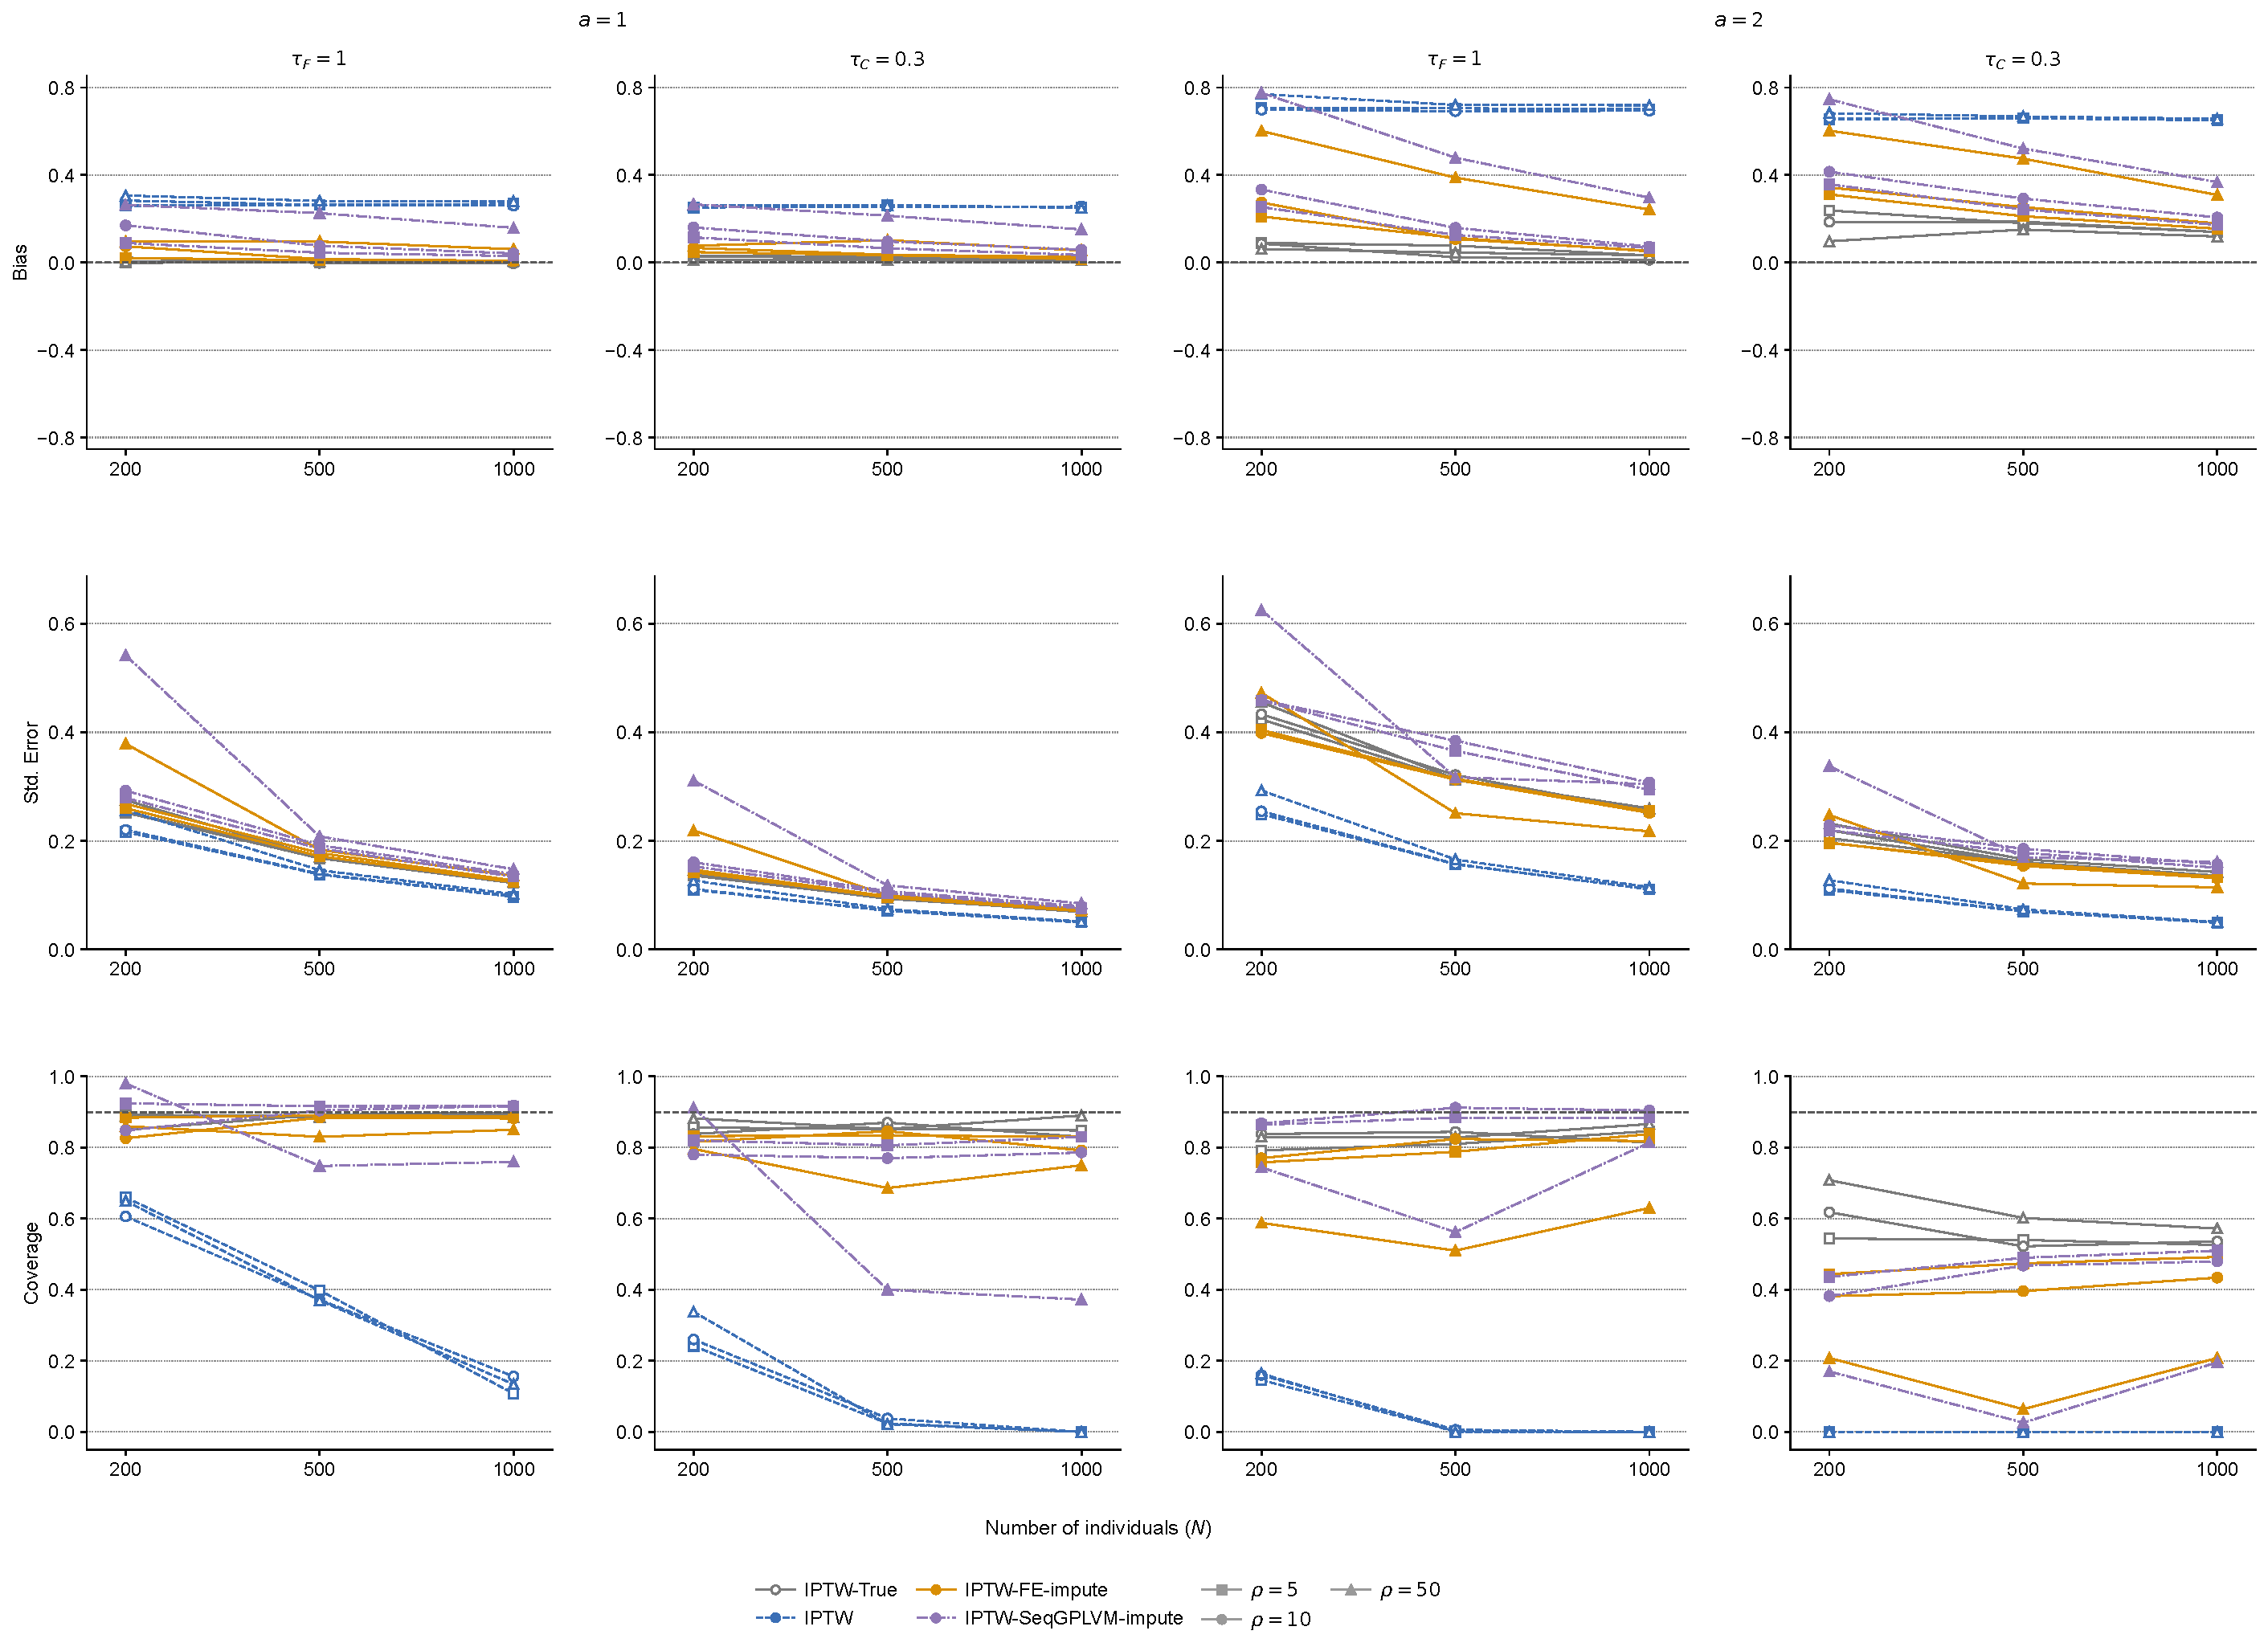
\includegraphics[width=1\textwidth]{figures/build/simulation_results.pdf}
    \caption{Simulation results for FE-MSM and sequential GPLVM.}
    \label{fig:simulation_results}
\end{figure}
\textbf{DISCUSSION}
\hl{While this MI-style propagation provides a principled empirical uncertainty summary,
it does not close the main theoretical gap in the sequential deconfounding approach.
First, it does not by itself deliver a large-sample result for the \emph{overall}
two-stage estimator---i.e., conditions under which the plug-in (or draw-averaged)
MSM estimator is consistent and $\sqrt{N}$-asymptotically normal with a valid variance
formula---of the kind established for FE--IPTW by Blackwell and Yamauchi.
Second, because the outcome stage is not modeled jointly with the treatment model,
the distribution of $\{\hat{\gamma}^{(s)}\}$ should be interpreted as uncertainty
propagation rather than a coherent Bayesian posterior for $\gamma$; consequently,
interval calibration is not automatically guaranteed from Bayesian first principles.
Third, even perfect variance combination does not address potential sources of
systematic error---such as misspecification of the latent treatment model/CMM,
violations of positivity leading to unstable weights, or approximation error from
variational inference---which can affect both bias and coverage.}
\chapter{Discussion}
\label{chap:discussion}

This thesis aimed to clarify the assumptions and the finite-sample performance of two 
approaches to address 
time-constant unmeasured confounding in the context of time-varying treatments. 
Although the simulation results show improvements in the bias of the 
causal effect estimates for both methods, there are still some limitations and 
open questions which make these methods not yet ready for 
widespread use in practice. The fundamental requirement behind both of these methods 
is another form of ignorability assumption which includes a time-invariant latent variable 
in the conditioning set which make the treatment assignment independent of the potential 
outcomes. 

In FE-MSM this requirement is directly assumed and is formalized by 
Assumption~\ref{ass:FE-unit-specific-ignor}. The restriction they put in this assumption 
on the unmeasured confounder is that using a latent scalar variable $\alpha_i$, 
all the 
time-invariant unmeasured confounding in the treatment process 
can be captured. Effectively, this assumption restricts the class 
of DGPs which this method can address to the class of DGPs where the unmeasured confounder 
only enters the treatment process as a scalar or, at least, where those confounders can be summarized 
into one scalar. This is a strong structural assumption which cannot be verified 
using observed data. For instance, this method cannot be used in cases where 
the unmeasured confounding modifies not only the intercept but also 
the effect of other covariates or treatments (interaction effects). 

On the other hand, in SeqGPLVM, this requirement 
is justified by means of assuming a set of auxiliary 
assumptions (Assumptions~\ref{ass:SG-Marcovianity}-\ref{ass:SG-Consistency}). 
Among these assumptions, the assumption of consistency of the latent variable 
plays the most crucial role. This assumption is not only impossible to verify in 
real-world problems, but it is not straightforward to establish even in simulation studies where 
the DGP is known. To verify this assumption for a given DGP, one would need to show that the 
relevant latent confounder is uniquely identified, up to trivial transformations, 
by the observed data. Note that the notion of identifiability considered here 
is closer to structural identifiability, since the issue is whether the 
latent confounder is uniquely implied by the data-generating structure, 
rather than whether a parameter can be estimated within a fixed statistical model. 
This is a much 
stronger requirement than merely showing that there exists some latent-variable representation 
of the treatment process. In general, different latent structures may induce the same observed 
distribution of the treatments, and therefore the same observed data may be compatible with 
multiple candidate substitute confounders. In such a case, even if a latent-variable model fits 
the treatment process well, it does not follow that the recovered latent variable corresponds to 
the confounder needed for causal identification. In other words, SeqGPLVM 
may recover a latent factor that explains the dependence structure among the treatments, 
but this alone does not guarantee that this latent factor is the correct one for the 
causal problem. This is a fundamental issue for all methods that rely on latent 
variable models for deconfounding, and it is not specific to SeqGPLVM.

Consequently, the favorable simulation results for SeqGPLVM should be 
interpreted with caution. This method is shown to work in a specific DGP and for larger 
sample sizes, but the satisfaction of the concistency assumption is left for 
future work. More broadly, the method shifts the 
burden of the usual sequential ignorability assumption to a different and 
arguably less transparent set of 
structural assumptions about the existence, uniqueness, and causal relevance of a 
latent substitute 
confounder. Despite these theoretical limitations, the flexibility of SeqGPLVM 
in modeling complex relationships 
between the observed covariates, treatments, and the latent confounder for longitudinal data, 
can be studied further as a non-parametric latent variable model for time series data. 

A future direction is to add dynamics to the latent variable structure. Also another 
interesting direction is to implement an amortized version of SeqGPLVM which can 
be more efficient for new data by parametrizing the posterior distribution over the 
latent variables using a neural network.

In conclusion this thesis provided a common framework for understanding the assumptions 
and the finite-sample performance of two methods for addressing time-constant unmeasured 
confounding in time-varying treatments settings. 
It highlighted the assumptions and limitations of these methods and 
the need for further theoretical and empirical work to understand their 
properties and applicability. The results of this thesis suggested 
evidence that both FE-MSM and SeqGPLVM perform similarly for longer treatment sequences.  The 
results of this thesis provided emperical evidence that both FE-MSM 
and SeqGPLVM can be useful tools for addressing time-constant unmeasured confounding in 
certain settings to reduce bias and improve coverage compared to standard methods 
that do not account for unmeasured confounding. A promising future research 
direction is to 
investigate the theoretical properties of the fixed effects estimates by FE-MSM and the 
latent variables estimated by SeqGPLVM to understand the nature of these estimates 
and their relationship to the true unmeasured confounder. This could be pursued by 
further exploring the performance and the estimation of the latent variables 
and the fixed effects 
in simulation studies using alternative DGPs 
that impose a richer structure on the unmeasured confounding. 
For example, one could consider 
a hierarchical DGP in which individuals are first assigned to latent 
classes and the unmeasured confounder 
is then generated conditional on class membership. Such a design would 
induce structured heterogeneity in 
the population and would make it possible to investigate whether the fixed effects 
in FE-MSM and the latent 
variables inferred by SeqGPLVM recover only coarse subgroup structure or a 
quantitatively meaningful 
approximation to the underlying confounder. 
In this sense, the simulation framework suggested by 
\citeA{bouchattaouiCausalDynamicVariational2025} may provide a useful starting point, 
even though that 
paper focuses on unobserved adjustment variables rather than unobserved confounders.

Another idea inspired by \citeA{bouchattaouiCausalDynamicVariational2025} is to investigate 
whether the consistency assumption for SeqGPLVM can be imposed also in practice by imposing 
a more concentrated,
approximately deterministic posterior over the latent variables. 
The theory of deconfounding requires 
that the latent substitute confounder is a deterministic function of the 
treatment sequence 
while in practice the posterior distribution over the latent variables is 
typically diffuse, especially for smaller sample sizes. If successful, 
such an approach could lead 
to more stable latent representations 
and reduce the sensitivity of the resulting causal effect estimates to 
posterior uncertainty in the inferred confounder.

\begin{comment}
\textbf{DISCUSSION}
\hl{While this MI-style propagation provides a principled empirical uncertainty summary,
it does not close the main theoretical gap in the sequential deconfounding approach.
First, it does not by itself deliver a large-sample result for the \emph{overall}
two-stage estimator---i.e., conditions under which the plug-in (or draw-averaged)
MSM estimator is consistent and $\sqrt{N}$-asymptotically normal with a valid variance
formula---of the kind established for FE--IPTW by Blackwell and Yamauchi.
Second, because the outcome stage is not modeled jointly with the treatment model,
the distribution of $\{\hat{\gamma}^{(s)}\}$ should be interpreted as uncertainty
propagation rather than a coherent Bayesian posterior for $\gamma$; consequently,
interval calibration is not automatically guaranteed from Bayesian first principles.
Third, even perfect variance combination does not address potential sources of
systematic error---such as misspecification of the latent treatment model/CMM,
violations of positivity leading to unstable weights, or approximation error from
variational inference---which can affect both bias and coverage.}


\begin{itemize}
    \item discuss about the vocablurary choice of "unmeasured" vs "hidden"
    \item testing against misspecified latent space dimension (I think bica does this?)
    \item implications of having one GP per time step vs one big GP for all time steps (maybe cite 
    some GP time series work?)
    \item discuss the none parametric nature of GP and its implications, specifically in the context of IPTW and the assumption of correct propensity model specification
    \item discuss about the amortized version of GPLVM (perhaps in the appendix)
    \item \hl{what} \cite{hattSequentialDeconfoundingCausal2024} \hl{did seems very wrong. it seems that they extract the latent variables from the treatment model and then use them as if they were observed covariates in the MSM. The worrisome part is that they are using IPTW which means after extracting the esimated latent substitute, they fit another propensity model incluing the estimated treatments so basically on the left hand side we have $a_it$ and the on the right hand side we have a function of $a_it$. This seems very wrong. We should discuss this. What I did, which seems more correct, is to use the estimated propensities from the seqgplvm treatment model directly in the MSM. Althoughm, this can also cause some problems because seqgplvm is a very powerful model and it can overfit the treatment assignment and lead to extreme weights.}
    \item another break point of this whole story of deconfounding with latent variables is the assumption of pinpointability. in the context of the time varying treatments, this assumption means that the latent variables estimated should stay the same for all hypothetical treatment assignments. I need to read D'amor critique of deconfounding paper again. 
    \item another big issue is that, their second propensity model is the msm stage is not even correctly specified! Although they removed the explicit equations they used for the MSM stage, from their previous version, I remeber that they used a model that was not the same as the DGP. 
    \item Another point is that, the selling point of Hatt et al was that SeqGPLVM is flexible in terms of 
    captuing non linear relationships between the latent confounders, observed covariates and treatment assignments. However, 
    because of the pinpointability assumption, there is a high chance that the those more complicated relationships in the dgp, 
    cannot satisfied the pinpointability assumption. It would be nice if I can find a dgps that is not very complicated but 
    violates the pinpointability assumption. Maybe reading D'amor critique paper again can help with this.
    \item discuss about the SeqGPLVM architecture choice of having separate parameters for each time step vs having shared parameters across time steps and its
    implications. Note that this is not the most efficient way to parameterize a time series model if we believe that the dgp's paramters do not change over time.  
    \item discuss about the big assumption \cite{blackwellEffectPoliticalAdvertising2024} 
    make about $Z_i = f(U_i)$ and perhaps what effectively \cite{hattSequentialDeconfoundingCausal2024} 
    is doing to not assume this but instead in their theorwm 1, they are tyring to show that 
    their $Z_i$, is enough to retain the sequential ignorability assumption. But a future 
    direction is to investigate if one results in another in the sense that if 
    $Z_i$ is enough to retain the sequential ignorability assumption, then it must be the case that $Z_i = f(U_i)$ for some function $f$.
    \item advantage using seqgplvm is that it let the uncertainty in the 
    estimation of propensity scores to be propagated to the final 
    estimation of the causal effect. 

    \item in this work we show via simulations that SeqGPLVM can result in similar results as 
    FE-MSM and this motivates to work on the consistency theory of SeqGPLVM similar to 
    what \cite{blackwellEffectPoliticalAdvertising2024} did for FE-MSM. more specifically, 
    we need to show that the propensity scores estimated by SeqGPLVM are 
    consistent estimates of the true propensity scores. 

    \item discuss that it would be better if we use the amortized version of 
    SeqGPLVM since now for new data we need to refit only the part of the model 
    corresponding to the latent variable while freezing the rest of the parameters. 
    but via amortized inference, we can directly get the latent variable for new data without refitting any part of the model.
\end{itemize}

\section{Problem of reusing the estimated latent variables in a second stage outcome model involving propensity score estimation}
\label{sec:hatt-problems}
As mentioned in section \ref{sec:seqgplvm}, in \cite{hattSequentialDeconfoundingCausal2024}, the authors treat 
SeqGPLVM as a factor model whose purpose is to estimate the posterior over the latent confounder substitutes, 
\(p(\mathbf{z}_i \mid \bar{a}_{iT}, \bar{\mathbf{x}}_{iT})\). Then, the authors proceed to use samples 
from this posterior distribution as if they were observed covariates in a second stage outcome model. 
Specifically, they suggest fitting two propensity score based models: 
marginal structural model (MSM)\cite{robinsEstimationCausalEffects2008} and 
Recurrent Marginal Structural Networks \cite{limForecastingTreatmentResponses2018}. The 
problem with this approach is that in both of these models, the authors fit a second propensity score model 
that includes the estimated confounder substitutes \(\mathbf{z}_i\) as covariates. However, since \(\mathbf{z}_i\) 
are estimated from the treatment assignments \(\bar{a}_{iT}\), including them as covariates in a second propensity score 
model that aims to predict \(\bar{a}_{iT}\) creates a circular dependency. More concretely, 
in the second stage propensity score model, we are trying to estimate 
\(p(A_{it} \mid \bar{A}_{i,t-1}, \bar{\mathbf{X}}_{it}, \mathbf{z}_i)\) where \(\mathbf{z}_i\) is a function of 
\(\bar{a}_{iT}\) and \(\bar{x}_{iT}\). 
This circular dependency can lead to biased estimates of
using inverse probability of treatment weighting (IPTW), where the propensity scores are estimated by including the estimated confounder substitutes $\mathbf{z}_i$ as covariates.

Also note that the correct way of using the posterior distribution over 
the latent confounder substitutes \(p(\mathbf{z}_i \mid \bar{a}_{iT}, \bar{\mathbf{x}}_{iT})\)
is to integrate over this distribution when estimating the causal effect, i.e.,
\begin{equation}
    \mathbb{E}\left[Y_{iT}(\bar{d}_{T-k:T})\right] = \int \mathbb{E}\left[Y_{iT}(\bar{d}_{T-k:T}) \mid \mathbf{z}_i\right] p(\mathbf{z}_i \mid \bar{a}_{iT}, \bar{\mathbf{x}}_{iT}) d\mathbf{z}_i
\end{equation}
which can be approximated using Monte Carlo integration by drawing samples from the posterior distribution, 
calculate the conditional propensity scores by the SeqGPLVM likelihood for the 
observed treatment, and then use these propensity scores in the IPTW estimation of the MSM.
Repeat this for multiple samples from the posterior and average the results to obtain the final estimate of the causal effect. 

Note that in \cite{bicaTimeSeriesDeconfounder2020} and \cite{wangBlessingsMultipleCauses2019} 
They also follow a similar two stage procedure where they first estimate the latent confounders
using a factor model and then use these estimated confounders as observed covariates in the outcome model. 
However, they do not use IPTW for estimating the causal effect in the outcome model. 
Instead, they use G-formula which does not involve fitting a second propensity score model.
\end{comment}

\bibliographystyle{apacite}
\bibliography{references}
\clearpage
\appendix
\chapter{Proof of Theorem 1}
\label{proof_theorem_1}
The appendix of \citeA{hattSequentialDeconfoundingCausal2024} 
formulates the proof for Theorem 1 only for a first-order
conditional Markov model over treatments. 
However, the same proof strategy extends naturally
to finite order \(p\) by augmenting the treatment state with the 
last \(p\) treatments. The
result below is therefore a straightforward extension
of their recursive-construction argument. 

\begin{proposition}[Finite-order extension of the proof strategy of \citeA{hattSequentialDeconfoundingCausal2024}]
Suppose that for some fixed integer \(p \ge 1\), the assigned treatment process satisfies
the conditional Markov property of order \(p\), that is,
\begin{equation}
\label{eq:p-order-cmm}
p_{\boldsymbol{\gamma}}(\bar{\mathbf{a}}_{iT}\mid \bar{\mathbf{x}}_{iT},\mathbf{z}_i)
=
\prod_{t=1}^T
p_{\boldsymbol{\gamma}_t}(a_{it}\mid \mathbf{a}_{i,t-p:t-1},\bar{\mathbf{x}}_{it},\mathbf{z}_i),
\end{equation}
where \(\mathbf{a}_{i,t-p:t-1}=(a_{i,t-p},\dots,a_{i,t-1})\), with the convention that for \(t<1\),
\(a_{it}=0\). Assume further that the treatment space is a Borel space and that unobserved
confounding is time-invariant in the sense maintained by \citeA{hattSequentialDeconfoundingCausal2024}.

Then the proof strategy of \citeA{hattSequentialDeconfoundingCausal2024} extends to yield a recursive representation
\begin{equation}
\label{eq:p-order-recursion}
A_{it} = f_t(\mathbf{A}_{i,t-p:t-1},\mathbf{Z}_i,\bar{\mathbf{X}}_{it},V_{it}),
\end{equation}
where \(V_{it} \sim \mathrm{Uniform}([0,1])\), and
\begin{equation}
\label{eq:p-order-v-indep}
V_{it} \perp Y_i(\bar{\mathbf{a}}_t)\mid \bar{\mathbf{A}}_{i,t-1},\bar{\mathbf{X}}_{it},\mathbf{Z}_i
\qquad
\text{for all } \bar{\mathbf{a}}_t \in \bar{\mathcal A}_t.
\end{equation}
Consequently,
\begin{equation}
\label{eq:p-order-ssi}
A_{it} \perp Y_i(\bar{\mathbf{a}}_t)\mid \bar{\mathbf{A}}_{i,t-1},\bar{\mathbf{X}}_{it},\mathbf{Z}_i
\qquad
\text{for all } \bar{\mathbf{a}}_t \in \bar{\mathcal A}_t.
\end{equation}
\end{proposition}

\begin{proof}
The argument follows the same structure as the appendix of \citeA{hattSequentialDeconfoundingCausal2024}, but
with a state augmentation step.

First, define the augmented treatment state
\[
\mathbf{S}_{it} := (A_{i,t-p+1},\dots, A_{it}) \in \mathcal A^p.
\]
Under \eqref{eq:p-order-cmm}, the treatment process is Markov of order \(p\) conditional on
\((\bar{\mathbf{X}}_{it},\mathbf{Z}_i)\). Equivalently, the augmented state process \((\mathbf{S}_{it})_{t\ge1}\) is first-order
Markov conditional on \((\bar{\mathbf{X}}_{it},\mathbf{Z}_i)\). Indeed, for each \(t\),
\[
\mathbb{P}(\mathbf{S}_{it} \in B \mid \bar{\mathbf{S}}_{i,t-1}, \bar{\mathbf{X}}_{it}, \mathbf{Z}_i)
=
\mathbb{P}(\mathbf{S}_{it} \in B \mid \mathbf{S}_{i,t-1}, \bar{\mathbf{X}}_{it}, \mathbf{Z}_i)
\]
for all measurable \(B \subseteq \mathcal A^p\), because the first \(p-1\) coordinates of
\(\mathbf{S}_{it}\) are deterministic shifts of \(\mathbf{S}_{i,t-1}\), while the last coordinate \(A_{it}\) depends
on the past only through \(\mathbf{A}_{i,t-p:t-1}\), \(\bar{\mathbf{X}}_{it}\), and \(\mathbf{Z}_i\).

Since \(\mathcal A^p\) is again a Borel space, the same Kallenberg recursion argument used by
\citeA{hattSequentialDeconfoundingCausal2024} for the order-1 case applies to the augmented state process.
Therefore, there exist measurable functions \(F_t\) and i.i.d. random variables
\(V_{it} \sim \mathrm{Uniform}([0,1])\) such that
\[
\mathbf{S}_{it} = F_t(\mathbf{S}_{i,t-1}, \mathbf{Z}_i, \bar{\mathbf{X}}_{it}, V_{it}).
\]
Let \(f_t\) denote the last-coordinate projection of \(F_t\). Then
\[
A_{it} = f_t(\mathbf{A}_{i,t-p:t-1}, \mathbf{Z}_i, \bar{\mathbf{X}}_{it}, V_{it}),
\]
which establishes \eqref{eq:p-order-recursion}.

It remains to verify \eqref{eq:p-order-v-indep}. This is the same step that remains to be shown
in the proof of Lemma 2 in \citeA{hattSequentialDeconfoundingCausal2024}. Their argument extends without essential
change. Suppose, for contradiction, that there exists an omitted variable $W$ that confounds
\(V_{it}\) and \(Y_i(\bar{\mathbf{a}}_t)\) conditional on \((\bar{\mathbf{A}}_{i,t-1},\bar{\mathbf{X}}_{it},\mathbf{Z}_i)\). 
Moreover, according to Assumption~\ref{ass:SG-No-single-time-point-confounding}, there is no 
single-time confounders. Hence, $W$ at least affect $V_{is}$ where $s \neq t$. 
But the recursion construction yields that the \(V_{it}\) are i.i.d. Uniform\([0,1]\),
so such a common time-invariant source of dependence is excluded. 
If instead the omitted variable is time-varying, then because
\[
A_{it} = f_t(\mathbf{A}_{i,t-p:t-1}, \mathbf{Z}_i, \bar{\mathbf{X}}_{it}, V_{it}),
\]
the same omitted variable would induce confounding between \(A_{it}\) and \(Y_i(\bar{\mathbf{a}}_t)\).
This contradicts the maintained setup that any unobserved confounding is time-invariant and is
captured through the latent static variable \(\mathbf{Z}_i\). Hence,
\[
V_{it} \perp Y_i(\bar{\mathbf{a}}_t)\mid \bar{\mathbf{A}}_{i,t-1},\bar{\mathbf{X}}_{it},\mathbf{Z}_i,
\]
which proves \eqref{eq:p-order-v-indep}.

Finally, define
\[
\mathcal G_{it} := \sigma(\bar{\mathbf{A}}_{i,t-1},\bar{\mathbf{X}}_{it},\mathbf{Z}_i).
\]
Since \((\mathbf{A}_{i,t-p:t-1}, \mathbf{Z}_i, \bar{\mathbf{X}}_{it})\) is \(\mathcal G_{it}\)-measurable, \eqref{eq:p-order-v-indep}
implies
\[
(\mathbf{A}_{i,t-p:t-1}, \mathbf{Z}_i, \bar{\mathbf{X}}_{it}, V_{it}) \perp Y_i(\bar{\mathbf{a}}_t)\mid \mathcal G_{it}.
\]
Because \(A_{it}\) is a measurable function of \((\mathbf{A}_{i,t-p:t-1}, \mathbf{Z}_i, \bar{\mathbf{X}}_{it}, V_{it})\), conditional
independence is preserved under measurable transformations, and therefore
\[
A_{it} \perp Y_i(\bar{\mathbf{a}}_t)\mid \mathcal G_{it}.
\]
Equivalently,
\[
A_{it} \perp Y_i(\bar{\mathbf{a}}_t)\mid \bar{\mathbf{A}}_{i,t-1},\bar{\mathbf{X}}_{it},\mathbf{Z}_i.
\]
This proves \eqref{eq:p-order-ssi}.
\end{proof}

% ------------------------------------------------------------
% Appendix: Deriving the (negative) ELBO loss for the SeqGPLVM
% ------------------------------------------------------------

\section{SeqGPLVM loss function}
\label{sec:seqgplvm_loss}
In this section, we derive the ELBO (evidence lower bound) for the sequential Gaussian process latent variable 
model (SeqGPLVM) introduced in Section~\ref{sec:seqgplvm}. 

\subsection{Notation}
We use uppercase letters to denote random quantities and the 
corresponding lowercase letters to denote their realizations; boldface 
indicates vector or collection-valued objects, while plain letters denote 
scalars. Let \(\mathbf{X}_{it}\in\mathbb{R}^D\) denote the random covariate vector 
for individual \(i\) at time \(t\), and let \(\mathbf{x}_{it}\) denote its realization, 
where \(N\) is the number of individuals, \(D\) is the number of covariates, and \(T\) 
is the number of time points. Let \(A_{it}\in\{0,1\}\) denote the random treatment for 
individual \(i\) at time \(t\), and let \(a_{it}\) denote its realization. 
Here, we assume scalar treatments for simplicity, but the extension to multi-dimensional 
treatments is straightforward. Also, we assume a binary treatment for concreteness; 
however, this restriction is not required for the theoretical results. 
We index individuals by \(i \in \{1,\dots,N\}\) and time by \(t \in \{1,\dots,T\}\).

We let \(\mathbf{A}_t = \{A_{it}\}_{i=1}^N\) and \(\mathbf{X}_t = \{\mathbf{X}_{it}\}_{i=1}^N\) 
denote the collections of treatments and covariate vectors, respectively, 
for all individuals at time \(t\), and \(\mathbf{A}_i = \{A_{it}\}_{t=1}^T\) 
and \(\mathbf{X}_i = \{\mathbf{X}_{it}\}_{t=1}^T\) denote the corresponding 
random collections over all time points for individual \(i\). Their observed 
realizations are denoted by 
\(\mathbf{a}_t = \{a_{it}\}_{i=1}^N\), \(\mathbf{x}_t = 
\{\mathbf{x}_{it}\}_{i=1}^N\), \(\mathbf{a}_i = \{a_{it}\}_{t=1}^T\), 
and \(\mathbf{x}_i = \{\mathbf{x}_{it}\}_{t=1}^T\). Therefore, 
we write \(\mathbf{A} = \{\mathbf{A}_t\}_{t=1}^T = \{\mathbf{A}_i\}_{i=1}^N\) 
for the full random treatment collection and 
\(\mathbf{a} = \{\mathbf{a}_t\}_{t=1}^T = \{\mathbf{a}_i\}_{i=1}^N\) for its realization. 
Similarly, we write \(\mathbf{X} = \{\mathbf{X}_t\}_{t=1}^T = \{\mathbf{X}_i\}_{i=1}^N\) 
for the full random covariate collection and \(\mathbf{x} = \{\mathbf{x}_t\}_{t=1}^T = 
\{\mathbf{x}_i\}_{i=1}^N\) for its realization. We use \(\mathbf{Z} = \{\mathbf{Z}_i\}_{i=1}^N\) to denote the collection of time-invariant 
latent variables, where \(\mathbf{Z}_i \in \mathbb{R}^J\) is the 
latent variable for individual \(i\) and \(J\) is the latent dimensionality. 

We use \(\boldsymbol{\gamma}\) and \(\boldsymbol{\psi}\) to denote the 
generative and variational hyperparameters, respectively. Generative hyperparameters are 
those that define how the data is generated and enter the prior and likelihood, e.g., 
the kernel lengthscale and variance in GPs, while variational hyperparameters are those 
that define the variational family, e.g., the mean and variance in Gaussian variational 
distributions.

\subsection{Variational inference background}
\label{sec:variational_inference_background}
The ultimate inferential goal of the SeqGPLVM is to estimate the posterior distribution over 
the time-invariant latent substitute confounder \(\mathbf{Z}\) given the observed data 
\(\mathbf{x}\) and \(\mathbf{a}\). By Bayes' rule, we can write the posterior as a 
function of the likelihood and prior:
\[
p_{\boldsymbol{\gamma}}(\mathbf{z}\mid \mathbf{x},\mathbf{a})
=
\frac{
p_{\boldsymbol{\gamma}}(\mathbf{a}\mid \mathbf{x},\mathbf{z})\,
p_{\boldsymbol{\gamma}}(\mathbf{z}\mid \mathbf{x})
}{
p_{\boldsymbol{\gamma}}(\mathbf{a}\mid \mathbf{x})
}.
\]
where the denominator
\(
p_{\boldsymbol{\gamma}}(\mathbf{a}\mid \mathbf{x})
\)
(the \emph{marginal likelihood} / \emph{evidence}) is the normalizing constant. Note that 
we use \(\boldsymbol{\gamma}\) to parameterize both the likelihood and the prior to make 
the notation more concise, 
but in practice, they can have different hyperparameters.
Rewriting the logarithm of evidence as an 
integral over latent variables,  
\begin{equation}
\log p_{\boldsymbol{\gamma}}(\mathbf{a}\mid \mathbf{x}) = 
\log \int p_{\boldsymbol{\gamma}}(\mathbf{a},\mathbf{z}\mid \mathbf{x})\,\mathrm{d}\mathbf{z}.
\end{equation}
In latent-variable models this integral is typically intractable which means the 
posterior cannot be computed exactly; introducing a tractable variational density 
\(q_{\boldsymbol{\psi}}(\mathbf{z}\mid \mathbf{x})\) 
yields a lower bound on \(\log p_{\boldsymbol{\gamma}}(\mathbf{a}\mid\mathbf{x})\). 
The gap between this bound and the true log-evidence is a KL divergence to the true posterior, 
so maximizing the bound pushes \(q_{\boldsymbol{\psi}}(\mathbf{z}\mid \mathbf{x})\) 
towards \(p_{\boldsymbol{\gamma}}(\mathbf{z}\mid \mathbf{x},\mathbf{a})\). To see this, 
the marginal likelihood can be written as
\begin{align}
\log p_{\boldsymbol{\gamma}}(\mathbf{a}\mid \mathbf{x})
&= \log \int p_{\boldsymbol{\gamma}}(\mathbf{a},\mathbf{z}\mid \mathbf{x})\,\mathrm{d}\mathbf{z}
\nonumber\\
&= \log \int q_{\boldsymbol{\psi}}(\mathbf{z}\mid \mathbf{x})\,
\frac{p_{\boldsymbol{\gamma}}(\mathbf{a},\mathbf{z}\mid \mathbf{x})}{q_{\boldsymbol{\psi}}(\mathbf{z}\mid \mathbf{x})}\,
\mathrm{d}\mathbf{z}
\nonumber\\
&\ge \int q_{\boldsymbol{\psi}}(\mathbf{z}\mid \mathbf{x})
\log\frac{p_{\boldsymbol{\gamma}}(\mathbf{a},\mathbf{z}\mid \mathbf{x})}{q_{\boldsymbol{\psi}}(\mathbf{z}\mid \mathbf{x})}\,
\mathrm{d}\mathbf{z}
\;=:\; \mathcal{L}(\boldsymbol{\psi},\boldsymbol{\gamma}),
\label{eq:elbo-def}
\end{align}
where the inequality is Jensen's inequality. $\mathcal{L}(\boldsymbol{\psi},\boldsymbol{\gamma})$ 
is called the evidence lower bound (ELBO). The KL divergence 
between the variational distribution and the true posterior can be written as

\begin{align*}
    \mathrm{KL}\!\left(q_{\boldsymbol{\psi}}(\mathbf{z}\mid \mathbf{x})\,\|\,p_{\boldsymbol{\gamma}}(\mathbf{z}\mid \mathbf{x},\mathbf{a})\right)
    &= \int q_{\boldsymbol{\psi}}(\mathbf{z}\mid \mathbf{x}) \log\frac{q_{\boldsymbol{\psi}}(\mathbf{z}\mid \mathbf{x})}{p_{\boldsymbol{\gamma}}(\mathbf{z}\mid \mathbf{x},\mathbf{a})}\, \mathrm{d}\mathbf{z} \\
    &= \int q_{\boldsymbol{\psi}}(\mathbf{z}\mid \mathbf{x}) \left[ \log q_{\boldsymbol{\psi}}(\mathbf{z}\mid \mathbf{x}) - \log p_{\boldsymbol{\gamma}}(\mathbf{z}\mid \mathbf{x},\mathbf{a}) \right] \, \mathrm{d}\mathbf{z} \\
    &= \int q_{\boldsymbol{\psi}}(\mathbf{z}\mid \mathbf{x}) \left[ \log q_{\boldsymbol{\psi}}(\mathbf{z}\mid \mathbf{x}) - \log\frac{p_{\boldsymbol{\gamma}}(\mathbf{a},\mathbf{z}\mid \mathbf{x})}{p_{\boldsymbol{\gamma}}(\mathbf{a}\mid \mathbf{x})} \right] \, \mathrm{d}\mathbf{z} \\
    &= \log p_{\boldsymbol{\gamma}}(\mathbf{a}\mid \mathbf{x}) - \int q_{\boldsymbol{\psi}}(\mathbf{z}\mid \mathbf{x}) \log\frac{p_{\boldsymbol{\gamma}}(\mathbf{a},\mathbf{z}\mid \mathbf{x})}{q_{\boldsymbol{\psi}}(\mathbf{z}\mid \mathbf{x})}\, \mathrm{d}\mathbf{z} \\
    &= \log p_{\boldsymbol{\gamma}}(\mathbf{a}\mid \mathbf{x}) - \mathcal{L}(\boldsymbol{\psi},\boldsymbol{\gamma}).
\end{align*}
Equivalently,
\begin{equation}
\log p_{\boldsymbol{\gamma}}(\mathbf{a}\mid \mathbf{x})
=
\mathcal{L}(\boldsymbol{\psi},\boldsymbol{\gamma})
+
\mathrm{KL}\!\left(q_{\boldsymbol{\psi}}(\mathbf{z}\mid \mathbf{x})\,\|\,p_{\boldsymbol{\gamma}}(\mathbf{z}\mid \mathbf{x},\mathbf{a})\right).
\label{eq:logp-decomp}
\end{equation}
Maximizing \(\mathcal{L}(\boldsymbol{\psi},\boldsymbol{\gamma})\) w.r.t.\ \(q\) minimizes the 
KL divergence to the true posterior and equality 
holds iff \(q_{\boldsymbol{\psi}}(\mathbf{z}\mid \mathbf{x}) = 
p_{\boldsymbol{\gamma}}(\mathbf{z}\mid \mathbf{x},\mathbf{a})\). 
This is true since the lhs of \eqref{eq:logp-decomp} does not depend on \(q\). 
Thus, we can use \(\mathcal{L}(\boldsymbol{\psi},\boldsymbol{\gamma})\) as a surrogate objective for approximate inference. 
\(\mathcal{L}(\boldsymbol{\psi},\boldsymbol{\gamma})\) can be rewritten as 
\begin{align}
\mathcal{L}(\boldsymbol{\psi},\boldsymbol{\gamma})
&= \int q_{\boldsymbol{\psi}}(\mathbf{z}\mid \mathbf{x})\,\log\!\left(\frac{p_{\boldsymbol{\gamma}}(\mathbf{a},\mathbf{z} \mid \mathbf{x})}{q_{\boldsymbol{\psi}}(\mathbf{z}\mid \mathbf{x})}\right)\, d\mathbf{z} \nonumber\\
&= \int q_{\boldsymbol{\psi}}(\mathbf{z}\mid \mathbf{x})\,\log p_{\boldsymbol{\gamma}}(\mathbf{a},\mathbf{z} \mid \mathbf{x})\, d\mathbf{z}
   \;-\; \int q_{\boldsymbol{\psi}}(\mathbf{z}\mid \mathbf{x})\,\log q_{\boldsymbol{\psi}}(\mathbf{z}\mid \mathbf{x})\, d\mathbf{z} \nonumber\\
&= \int q_{\boldsymbol{\psi}}(\mathbf{z}\mid \mathbf{x})\,\log\!\Big( p_{\boldsymbol{\gamma}}(\mathbf{a}\mid \mathbf{x},\mathbf{z})\,p_{\boldsymbol{\gamma}}(\mathbf{z}\mid \mathbf{x}) \Big)\, d\mathbf{z}
   \;-\; \int q_{\boldsymbol{\psi}}(\mathbf{z}\mid \mathbf{x})\,\log q_{\boldsymbol{\psi}}(\mathbf{z}\mid \mathbf{x})\, d\mathbf{z} \nonumber\\
&= \int q_{\boldsymbol{\psi}}(\mathbf{z}\mid \mathbf{x})\,\log p_{\boldsymbol{\gamma}}(\mathbf{a}\mid \mathbf{x},\mathbf{z})\, d\mathbf{z}
   \;-\; \int q_{\boldsymbol{\psi}}(\mathbf{z}\mid \mathbf{x})\,\log\!\left(\frac{q_{\boldsymbol{\psi}}(\mathbf{z}\mid \mathbf{x})}{p_{\boldsymbol{\gamma}}(\mathbf{z}\mid \mathbf{x})}\right)\, d\mathbf{z} \nonumber\\
&= \int q_{\boldsymbol{\psi}}(\mathbf{z}\mid \mathbf{x})\,\log p_{\boldsymbol{\gamma}}(\mathbf{a}\mid \mathbf{x},\mathbf{z})\, d\mathbf{z}
    \;-\; \mathrm{KL}\!\left(q_{\boldsymbol{\psi}}(\mathbf{z}\mid \mathbf{x})\,\|\,p_{\boldsymbol{\gamma}}(\mathbf{z}\mid \mathbf{x})\right)\nonumber\\
&= \mathbb{E}_{q_{\boldsymbol{\psi}}(\mathbf{z}\mid \mathbf{x})}\!\left[\log p_{\boldsymbol{\gamma}}(\mathbf{a}\mid \mathbf{x},\mathbf{z})\right]
    \;-\; \mathrm{KL}\!\left(q_{\boldsymbol{\psi}}(\mathbf{z}\mid \mathbf{x})\,\|\,p_{\boldsymbol{\gamma}}(\mathbf{z}\mid \mathbf{x})\right).
    \label{eq:elbo-rewrite}
\end{align}
Thus to setup variational inference, we need to specify the likelihood 
\(p_{\boldsymbol{\gamma}}(\mathbf{a}\mid \mathbf{x},\mathbf{z})\), 
the prior over latents \(p_{\boldsymbol{\gamma}}(\mathbf{z}\mid \mathbf{x})\), 
and the variational family \(q_{\boldsymbol{\psi}}(\mathbf{z}\mid \mathbf{x})\).

\subsection{Conditional markov model}
Let $\widetilde{\mathbf{X}}_t = \{(\bar{\mathbf{X}}_{it}, \mathbf{A}_{i,t-p:t-1}, 
\mathbf{Z}_i)\}_{i=1}^N$ be the augmented covariate vector at time $t$ 
that includes observed covariates history, the treatment history from time $t-p$ to $t-1$, 
and the latent substitute confounder. If the treatment assignments are 
generated according to a conditional Markov model of order $p$ then the 
likelihood in Eq.~\eqref{eq:elbo-rewrite} can be factorized as 
\begin{align}
p_{\boldsymbol{\gamma}}(\mathbf{a}\mid \mathbf{x},\mathbf{z}) = \prod_{t=1}^T p_{\gamma_t}(\mathbf{a}_{t} \mid \widetilde{\mathbf{x}}_{t}).
\end{align}
Substituting this factorization into the ELBO in Eq.~\eqref{eq:elbo-rewrite} yields
\begin{align}
    \label{eq:sequential_elbo}
\mathcal{L}(\boldsymbol{\psi},\boldsymbol{\gamma})= \mathbb{E}_{q_{\boldsymbol{\psi}}(\mathbf{z}\mid \mathbf{x})}\!\left[\sum_{t=1}^T \log p_{\boldsymbol{\gamma}_t}(\mathbf{a}_{t} \mid \widetilde{\mathbf{x}}_{t})\right]
    \;-\; \mathrm{KL}\!\left(q_{\boldsymbol{\psi}}(\mathbf{z}\mid \mathbf{x})\,\|\,p_{\boldsymbol{\gamma}}(\mathbf{z}\mid \mathbf{x})\right).
\end{align}

\subsection{Variational Inference for Bayesian Gaussian process latent variable models}
Bayesian Gaussian 
process latent variable models (GPLVMs) \cite{titsiasBayesianGaussianProcess2010} are 
a class of latent variable models that use Gaussian processes to model the relationship between observed data and latent variables. 
The term Bayesian is to distinguish it from the original 
GPLVM \cite{lawrenceGaussianProcessLatent2003} 
where the latent variables \( \mathbf{Z} \) are point estimated rather than 
inferred in a fully Bayesian manner. From now on, by GPLVMs we mean Bayesian GPLVMs. 
The idea behind GPLVMs is to model the relationship between the outcome and the 
observed covariates 
and the latent variables as a nonparametric function $f$ with a Gaussian process prior 
over it, 
\[
A_{it} \mid \widetilde{\mathbf{X}}_{it}, f_t
\sim p_t\!\left(\,\cdot \mid \boldsymbol{\theta}_{it}\right),
\qquad
g_t(\boldsymbol{\theta}_{it}) = f_t(\widetilde{\mathbf{X}}_{it}).
\]
where \(g_t\) is an appropriate link function and \(\boldsymbol{\theta}_{it}\)
denotes the parameter, or set of parameters, indexing the conditional distribution of $A_{it}$. 
The function \(f_t\) is a latent function 
in this framework, since it is not directly observed in the data.
Accordingly, it is assigned a prior distribution, namely a Gaussian process,
\[
f_t(\cdot) \sim \mathcal{GP}\!\left(m_t(\cdot), k_t(\cdot,\cdot;\boldsymbol{\gamma}_t)\right).
\]
where \(m_t(\cdot)\) is the mean function, \(k_t(\cdot, \cdot; \boldsymbol{\gamma}_t)\) 
is the kernel function parameterized by hyperparameters \(\boldsymbol{\gamma}_t\). 
They are 
both defined on the augmented input space. Let
\(
\mathbf{f}_t=\{f_t(\widetilde{\mathbf{x}}_{it})\}_{i=1}^N
\)
denote the vector of latent function values at these augmented inputs. 
The likelihood \(p_{\boldsymbol{\gamma}_t}(\mathbf{a}_{t}\mid 
\widetilde{\mathbf{x}}_{t})\)
is then obtained by marginalizing out the latent function values,
\begin{align}
p_{\boldsymbol{\gamma}_t}(\mathbf{a}_{t}\mid \widetilde{\mathbf{x}}_{t}) \nonumber
&=\int p_{\boldsymbol{\gamma}_t}(\mathbf{a}_{t}, \mathbf{f}_t\mid \widetilde{\mathbf{x}}_{t})\, d\mathbf{f}_t \nonumber \\ 
&=\int p_{\boldsymbol{\gamma}_t}(\mathbf{a}_{t}\mid \mathbf{f}_t, \widetilde{\mathbf{x}}_{t}) \, p(\mathbf{f}_t\mid \widetilde{\mathbf{x}}_{t})\, d\mathbf{f}_t \nonumber\\
&=\int p_{\boldsymbol{\gamma}_t}(\mathbf{a}_{t}\mid \mathbf{f}_t) \, p(\mathbf{f}_t\mid \widetilde{\mathbf{x}}_{t})\, d\mathbf{f}_t.
\label{eq:marginalized_over_f}
\end{align}
The last equality holds since the treatment is 
conditionally independent of the covariates and latent variables
given the latent function since the covariates only enter the likelihood through 
the latent function (see Figure~\ref{fig:seqgplvm_architecture}). Here, 
\(p(\mathbf{f}_t\mid \widetilde{\mathbf{x}}_t)\) is the GP prior over 
the vector of function values at the 
augmented inputs. 
If $p(\mathbf{a}_t\mid \mathbf{f}_t)$ is Gaussian, then 
the marginal likelihood can be computed in closed form: 
\[
p_{\boldsymbol{\gamma}_t}(\mathbf{a}_t\mid \widetilde{\mathbf{x}}_{t}) 
=\mathcal{N}\!\left(\mathbf{a}_t \mid m_t(\widetilde{\mathbf{x}}_t), k_t(\widetilde{\mathbf{x}}_t, \widetilde{\mathbf{x}}_t; \boldsymbol{\gamma}_t) + \sigma^2 \mathbf{I}\right). 
\]
However, in general, the likelihood is not Gaussian (e.g., binary treatments) 
and the integral in Eq.~\eqref{eq:marginalized_over_f} is intractable. In this 
case by introducing a variational distribution 
\(q_{\boldsymbol{\psi}_t}(\mathbf{f}_t\mid \widetilde{\mathbf{x}}_{t})\) 
and applying Jensen's inequality, we can obtain a lower 
bound on the log-likelihood at each time point:
\begin{align*}
\log p_{\boldsymbol{\gamma}_t}(\mathbf{a}_t\mid \widetilde{\mathbf{x}}_{t})
&= \log \int p_{\boldsymbol{\gamma}_t}(\mathbf{a}_t\mid \mathbf{f}_t) \, p(\mathbf{f}_t\mid \widetilde{\mathbf{x}}_{t})\, d\mathbf{f}_t \nonumber\\
&= \log \int q_{\boldsymbol{\psi}_t}(\mathbf{f}_t\mid \widetilde{\mathbf{x}}_{t}) \,
\frac{p_{\boldsymbol{\gamma}_t}(\mathbf{a}_t\mid \mathbf{f}_t) \, p(\mathbf{f}_t\mid \widetilde{\mathbf{x}}_{t})}
{q_{\boldsymbol{\psi}_t}(\mathbf{f}_t\mid \widetilde{\mathbf{x}}_{t})}\, d\mathbf{f}_t \nonumber\\
&\ge \int q_{\boldsymbol{\psi}_t}(\mathbf{f}_t\mid \widetilde{\mathbf{x}}_{t}) \,
\log\!\left(
\frac{p_{\boldsymbol{\gamma}_t}(\mathbf{a}_t\mid \mathbf{f}_t) \, p(\mathbf{f}_t\mid \widetilde{\mathbf{x}}_{t})}
{q_{\boldsymbol{\psi}_t}(\mathbf{f}_t\mid \widetilde{\mathbf{x}}_{t})}
\right)\, d\mathbf{f}_t \\
&= \mathbb{E}_{q_{\boldsymbol{\psi}_t}(\mathbf{f}_t\mid \widetilde{\mathbf{x}}_{t})}
\!\left[\log p_{\boldsymbol{\gamma}_t}(\mathbf{a}_t\mid \mathbf{f}_t)\right]
- \mathrm{KL}\!\left(
q_{\boldsymbol{\psi}_t}(\mathbf{f}_t\mid \widetilde{\mathbf{x}}_{t})
\,\big\|\,
p(\mathbf{f}_t\mid \widetilde{\mathbf{x}}_{t})
\right).
\end{align*}
This lower bound is true for all $t \in \{1, \ldots, T\}$. Hence the lower bound on 
the sum of log-likelihoods across all time points is
\begin{align*}
\sum_{t=1}^T \log p_{\boldsymbol{\gamma}_t}(\mathbf{a}_t\mid \widetilde{\mathbf{x}}_{t})
&\ge \sum_{t=1}^T \mathbb{E}_{q_{\boldsymbol{\psi}_t}(\mathbf{f}_t\mid \widetilde{\mathbf{x}}_{t})}
\!\left[\log p_{\boldsymbol{\gamma}_t}(\mathbf{a}_t\mid \mathbf{f}_t)\right]
- \sum_{t=1}^T \mathrm{KL}\!\left(
q_{\boldsymbol{\psi}_t}(\mathbf{f}_t\mid \widetilde{\mathbf{x}}_{t})
\,\big\|\,
p(\mathbf{f}_t\mid \widetilde{\mathbf{x}}_{t})
\right)
\end{align*}
Taking the expectation w.r.t.\ 
\(q_{\boldsymbol{\psi}}(\mathbf{z}\mid \mathbf{x})\) on both sides yields
\begin{align*}
\mathbb{E}_{q_{\boldsymbol{\psi}}(\mathbf{z}\mid \mathbf{x})}\!\left[\sum_{t=1}^T \log p_{\boldsymbol{\gamma}_t}(\mathbf{a}_t\mid \widetilde{\mathbf{x}}_{t})\right]
&\ge \sum_{t=1}^T \mathbb{E}_{q_{\boldsymbol{\psi}}(\mathbf{z}\mid \mathbf{x})}\!
\left[
    \mathbb{E}_{q_{\boldsymbol{\psi}_t}(\mathbf{f}_t\mid \widetilde{\mathbf{x}}_{t})}
    \!\left[\log p_{\boldsymbol{\gamma}_t}(\mathbf{a}_t\mid \mathbf{f}_t)\right]
\right] \\
&\quad
\;-\; 
    \sum_{t=1}^T \mathbb{E}_{q_{\boldsymbol{\psi}}(\mathbf{z}\mid \mathbf{x})} 
    \left[
    \mathrm{KL}\!\left(
    q_{\boldsymbol{\psi}_t}(\mathbf{f}_t\mid \widetilde{\mathbf{x}}_{t})
    \,\big\|\,
    p(\mathbf{f}_t\mid \widetilde{\mathbf{x}}_{t})
    \right)
    \right].
\end{align*}
Substituting this lower bound into the ELBO in Eq.~\eqref{eq:sequential_elbo} yields
\begin{align}
\mathcal{L}(\boldsymbol{\psi},\boldsymbol{\gamma}) 
&\ge \sum_{t=1}^T \mathbb{E}_{q_{\boldsymbol{\psi}}(\mathbf{z}\mid \mathbf{x})}
\!\left[\mathbb{E}_{q_{\boldsymbol{\psi}_t}(\mathbf{f}_t\mid \widetilde{\mathbf{x}}_{t})}
\!\left[\log p_{\boldsymbol{\gamma}_t}(\mathbf{a}_t\mid \mathbf{f}_t)\right]\right]\nonumber\\
&\quad
\;-\;
\sum_{t=1}^T \mathbb{E}_{q_{\boldsymbol{\psi}}(\mathbf{z}\mid \mathbf{x})} 
    \left[
    \mathrm{KL}\!\left(
    q_{\boldsymbol{\psi}_t}(\mathbf{f}_t\mid \widetilde{\mathbf{x}}_{t})
    \,\big\|\,
    p(\mathbf{f}_t\mid \widetilde{\mathbf{x}}_{t})
    \right)
    \right] \nonumber\\ 
&\quad
\;-\; \mathrm{KL}\!\left(q_{\boldsymbol{\psi}}(\mathbf{z}\mid \mathbf{x})\,\|\,p_{\boldsymbol{\gamma}}(\mathbf{z}\mid \mathbf{x})\right) = \widetilde{\mathcal{L}}(\boldsymbol{\psi}, \boldsymbol{\gamma}).
\label{eq:new_lower_bound}
\end{align}
Hence, 
\begin{equation}
\log p_{\boldsymbol{\gamma}}(\mathbf{a}\mid \mathbf{x})\ge 
\mathcal{L}(\boldsymbol{\psi}, \boldsymbol{\gamma}) 
\ge \widetilde{\mathcal{L}}(\boldsymbol{\psi}, \boldsymbol{\gamma}).
\label{eq:final_lower_bound}
\end{equation}
Thus, \(\widetilde{\mathcal{L}}(\boldsymbol{\psi}, \boldsymbol{\gamma})\) 
is a valid lower bound on the log-evidence and can be used as a 
surrogate objective for variational inference in the sequential GPLVM.

\subsection{Inducing points}

The lower bound in Eq.~\eqref{eq:new_lower_bound} still involves a variational
distribution over the full random vector of latent function values
\(\mathbf{f}_t \in \mathbb{R}^N\) at each time point \(t\). 
In Gaussian process models, this leads to computational costs
that scale poorly with the number of observations. 
To obtain a more scalable approximation, we introduce a set of 
\(M_t \ll N\) inducing inputs for each time point \(t\), 
\[ \mathbf{w}_t = \{\mathbf{w}_{mt}\}_{m=1}^{M_t}, \] 
defined on the same augmented input space as \(\widetilde{\mathbf{x}}_t\), 
together with the corresponding inducing variables 
\[ 
\mathbf{u}_t = \{f_t(\mathbf{w}_{mt})\}_{m=1}^{M_t}. 
\]
Under the Gaussian process prior, the joint distribution of the random latent
function values \(\mathbf{f}_t\) at the observed augmented inputs and the
inducing random variables \(\mathbf{u}_t\) is Gaussian:
\[
\begin{bmatrix}
\mathbf{f}_t\\
\mathbf{u}_t
\end{bmatrix}
\;\bigm|\;
\widetilde{\mathbf{x}}_t,\mathbf{w}_t
\sim
\mathcal{N}\!\left(
\begin{bmatrix}
\mathbf{m}_{\widetilde{\mathbf{x}},t}\\
\mathbf{m}_{\mathbf{w},t}
\end{bmatrix},
\begin{bmatrix}
\mathbf{K}^{(t)}_{\widetilde{\mathbf{x}}\widetilde{\mathbf{x}}} & \mathbf{K}^{(t)}_{\widetilde{\mathbf{x}}\mathbf{w}}\\
\mathbf{K}^{(t)}_{\mathbf{w}\widetilde{\mathbf{x}}} & \mathbf{K}^{(t)}_{\mathbf{w}\mathbf{w}}
\end{bmatrix}
\right),
\]
where
\[
\mathbf{m}_{\widetilde{\mathbf{x}},t} := m_t(\widetilde{\mathbf{x}}_t),
\qquad
\mathbf{m}_{\mathbf{w},t} := m_t(\mathbf{w}_t),
\]
and
\[
\mathbf{K}^{(t)}_{\widetilde{\mathbf{x}}\widetilde{\mathbf{x}}} := k_t(\widetilde{\mathbf{x}}_t,\widetilde{\mathbf{x}}_t;\boldsymbol{\gamma}_t),
\qquad
\mathbf{K}^{(t)}_{\widetilde{\mathbf{x}}\mathbf{w}} := k_t(\widetilde{\mathbf{x}}_t,\mathbf{w}_t;\boldsymbol{\gamma}_t),
\]
\[
\mathbf{K}^{(t)}_{\mathbf{w}\widetilde{\mathbf{x}}} := k_t(\mathbf{w}_t,\widetilde{\mathbf{x}}_t;\boldsymbol{\gamma}_t),
\qquad
\mathbf{K}^{(t)}_{\mathbf{w}\mathbf{w}} := k_t(\mathbf{w}_t,\mathbf{w}_t;\boldsymbol{\gamma}_t).
\]
It follows that
\[
p_{\boldsymbol{\gamma}_t}(\mathbf{f}_t,\mathbf{u}_t
\mid \widetilde{\mathbf{x}}_t,\mathbf{w}_t)
=
p_{\boldsymbol{\gamma}_t}(\mathbf{f}_t
\mid \mathbf{u}_t,\widetilde{\mathbf{x}}_t,\mathbf{w}_t)\,
p_{\boldsymbol{\gamma}_t}(\mathbf{u}_t\mid \mathbf{w}_t),
\]
where
\[
p_{\boldsymbol{\gamma}_t}(\mathbf{u}_t\mid \mathbf{w}_t)
=
\mathcal{N}\!\left(\mathbf{m}_{\mathbf{w},t},\mathbf{K}^{(t)}_{\mathbf{w}\mathbf{w}}\right),
\]
and
\begin{align}
p_{\boldsymbol{\gamma}_t}(\mathbf{f}_t
\mid \mathbf{u}_t,\widetilde{\mathbf{x}}_t,\mathbf{w}_t)
=
\mathcal{N}\!\Bigl(
&\mathbf{m}_{\widetilde{\mathbf{x}},t}
+
\mathbf{K}^{(t)}_{\widetilde{\mathbf{x}}\mathbf{w}}\bigl(\mathbf{K}^{(t)}_{\mathbf{w}\mathbf{w}}\bigr)^{-1}
(\mathbf{u}_t-\mathbf{m}_{\mathbf{w},t}),
\nonumber\\
&
\mathbf{K}^{(t)}_{\widetilde{\mathbf{x}}\widetilde{\mathbf{x}}}
-
\mathbf{K}^{(t)}_{\widetilde{\mathbf{x}}\mathbf{w}}\bigl(\mathbf{K}^{(t)}_{\mathbf{w}\mathbf{w}}\bigr)^{-1}\mathbf{K}^{(t)}_{\mathbf{w}\widetilde{\mathbf{x}}}
\Bigr).
\label{eq:f_conditional_u}
\end{align}
We now introduce a variational distribution over the inducing variables,
\[
q_{\boldsymbol{\psi}_t}(\mathbf{u}_t)
=
\mathcal{N}(\boldsymbol{\mu}_t,\mathbf{S}_t),
\]
and define the sparse variational family by
\[
% EDIT: the induced distribution over function values depends on both \psi_t and \gamma_t
q_{\boldsymbol{\psi}_t,\boldsymbol{\gamma}_t}(\mathbf{f}_t,\mathbf{u}_t\mid \widetilde{\mathbf{x}}_t)
=
p_{\boldsymbol{\gamma}_t}(\mathbf{f}_t\mid \mathbf{u}_t,\widetilde{\mathbf{x}}_t,\mathbf{w}_t)\,
q_{\boldsymbol{\psi}_t}(\mathbf{u}_t).
\]
Marginalizing over \(\mathbf{u}_t\) gives the implied variational distribution
over the latent function values,
\[
q_{\boldsymbol{\psi}_t,\boldsymbol{\gamma}_t}(\mathbf{f}_t\mid \widetilde{\mathbf{x}}_t)
=
\int
p_{\boldsymbol{\gamma}_t}(\mathbf{f}_t\mid \mathbf{u}_t,\widetilde{\mathbf{x}}_t,\mathbf{w}_t)\,
q_{\boldsymbol{\psi}_t}(\mathbf{u}_t)\,d\mathbf{u}_t.
\]
Using this variational family, the log-likelihood term at time \(t\) can be written as
\begin{align}
\log p_{\boldsymbol{\gamma}_t}(\mathbf{a}_t\mid \widetilde{\mathbf{x}}_t)
&=
\log \iint
p_{\boldsymbol{\gamma}_t}(\mathbf{a}_t\mid \mathbf{f}_t)\,
p_{\boldsymbol{\gamma}_t}(\mathbf{f}_t\mid \mathbf{u}_t,\widetilde{\mathbf{x}}_t,\mathbf{w}_t)\,
p_{\boldsymbol{\gamma}_t}(\mathbf{u}_t\mid \mathbf{w}_t)\,
d\mathbf{f}_t\,d\mathbf{u}_t
\nonumber\\
&=
\log \iint
q_{\boldsymbol{\psi}_t}(\mathbf{u}_t)\,
p_{\boldsymbol{\gamma}_t}(\mathbf{f}_t\mid \mathbf{u}_t,\widetilde{\mathbf{x}}_t,\mathbf{w}_t)\,
\frac{
p_{\boldsymbol{\gamma}_t}(\mathbf{a}_t\mid \mathbf{f}_t)\,
p_{\boldsymbol{\gamma}_t}(\mathbf{u}_t\mid \mathbf{w}_t)
}{
q_{\boldsymbol{\psi}_t}(\mathbf{u}_t)
}
\,d\mathbf{f}_t\,d\mathbf{u}_t
\nonumber\\
&\ge
\iint
q_{\boldsymbol{\psi}_t}(\mathbf{u}_t)\,
p_{\boldsymbol{\gamma}_t}(\mathbf{f}_t\mid \mathbf{u}_t,\widetilde{\mathbf{x}}_t,\mathbf{w}_t)
\log\!\left(
\frac{
p_{\boldsymbol{\gamma}_t}(\mathbf{a}_t\mid \mathbf{f}_t)\,
p_{\boldsymbol{\gamma}_t}(\mathbf{u}_t\mid \mathbf{w}_t)
}{
q_{\boldsymbol{\psi}_t}(\mathbf{u}_t)
}
\right)
d\mathbf{f}_t\,d\mathbf{u}_t
\nonumber\\
&=
\mathbb{E}_{q_{\boldsymbol{\psi}_t,\boldsymbol{\gamma}_t}(\mathbf{f}_t\mid \widetilde{\mathbf{x}}_t)}
\!\left[
\log p_{\boldsymbol{\gamma}_t}(\mathbf{a}_t\mid \mathbf{f}_t)
\right]
-
\mathrm{KL}\!\left(
q_{\boldsymbol{\psi}_t}(\mathbf{u}_t)
\,\big\|\,
p_{\boldsymbol{\gamma}_t}(\mathbf{u}_t\mid \mathbf{w}_t)
\right).
\label{eq:svgp_single_time_bound}
\end{align}
The last equality follows by marginalizing over \(\mathbf{u}_t\) to obtain
\[
q_{\boldsymbol{\psi}_t,\boldsymbol{\gamma}_t}(\mathbf{f}_t\mid \widetilde{\mathbf{x}}_t)
=
\int
p_{\boldsymbol{\gamma}_t}(\mathbf{f}_t\mid \mathbf{u}_t,\widetilde{\mathbf{x}}_t,\mathbf{w}_t)\,
q_{\boldsymbol{\psi}_t}(\mathbf{u}_t)\,d\mathbf{u}_t,
\]
and by using
\[
\int
p_{\boldsymbol{\gamma}_t}(\mathbf{f}_t\mid \mathbf{u}_t,\widetilde{\mathbf{x}}_t,\mathbf{w}_t)\,
d\mathbf{f}_t = 1.
\]
Substituting the bound in Eq.~\eqref{eq:svgp_single_time_bound} into
Eq.~\eqref{eq:sequential_elbo}, we obtain
\begin{align}
\mathcal{L}(\boldsymbol{\psi},\boldsymbol{\gamma})
&\ge
\sum_{t=1}^T
\mathbb{E}_{q_{\boldsymbol{\psi}}(\mathbf{z}\mid \mathbf{x})}
\!\left[
% EDIT: same notation correction here
\mathbb{E}_{q_{\boldsymbol{\psi}_t,\boldsymbol{\gamma}_t}(\mathbf{f}_t\mid \widetilde{\mathbf{x}}_t)}
\!\left[
\log p_{\boldsymbol{\gamma}_t}(\mathbf{a}_t\mid \mathbf{f}_t)
\right]
\right]
\nonumber\\
&\quad
-
\sum_{t=1}^T
\mathrm{KL}\!\left(
q_{\boldsymbol{\psi}_t}(\mathbf{u}_t)
\,\big\|\,
p_{\boldsymbol{\gamma}_t}(\mathbf{u}_t\mid \mathbf{w}_t)
\right)
-
\mathrm{KL}\!\left(
q_{\boldsymbol{\psi}}(\mathbf{z}\mid \mathbf{x})
\,\big\|\,
p_{\boldsymbol{\gamma}}(\mathbf{z}\mid \mathbf{x})
\right).
\label{eq:seqgplvm_inducing_bound}
\end{align}
Define
\begin{align}
\mathcal{L}_{\mathrm{ind}}(\boldsymbol{\psi},\boldsymbol{\gamma})
:=
&\sum_{t=1}^T
\mathbb{E}_{q_{\boldsymbol{\psi}}(\mathbf{z}\mid \mathbf{x})}
\!\left[
\mathbb{E}_{q_{\boldsymbol{\psi}_t,\boldsymbol{\gamma}_t}(\mathbf{f}_t\mid \widetilde{\mathbf{x}}_t)}
\!\left[
\log p_{\boldsymbol{\gamma}_t}(\mathbf{a}_t\mid \mathbf{f}_t)
\right]
\right]
\nonumber\\
&-
\sum_{t=1}^T
\mathrm{KL}\!\left(
q_{\boldsymbol{\psi}_t}(\mathbf{u}_t)
\,\big\|\,
p_{\boldsymbol{\gamma}_t}(\mathbf{u}_t\mid \mathbf{w}_t)
\right)
-
\mathrm{KL}\!\left(
q_{\boldsymbol{\psi}}(\mathbf{z}\mid \mathbf{x})
\,\big\|\,
p_{\boldsymbol{\gamma}}(\mathbf{z}\mid \mathbf{x})
\right).
\label{eq:inducing_elbo_def}
\end{align}
Then
\begin{equation}
\log p_{\boldsymbol{\gamma}}(\mathbf{a}\mid \mathbf{x})
\ge
\mathcal{L}(\boldsymbol{\psi},\boldsymbol{\gamma})
\ge
\mathcal{L}_{\mathrm{ind}}(\boldsymbol{\psi},\boldsymbol{\gamma}).
\label{eq:inducing_final_bound}
\end{equation}
Hence, \(\mathcal{L}_{\mathrm{ind}}(\boldsymbol{\psi},\boldsymbol{\gamma})\) is a valid
lower bound on the log-evidence and can be used as the optimization objective
for sparse variational inference in the SeqGPLVM. Equivalently, in practice one
minimizes the negative inducing-point ELBO,
\[
\mathcal{J}_{\mathrm{SeqGPLVM}}
=
-\mathcal{L}_{\mathrm{ind}}(\boldsymbol{\psi},\boldsymbol{\gamma}).
\]

Compared with the bound in Eq.~\eqref{eq:new_lower_bound}, 
this bound offers two key advantages. The expected log-likelihood is 
computed with respect to the sparse marginal posterior 
\(q_{\boldsymbol{\psi}_t,\boldsymbol{\gamma}_t}(\mathbf{f}_t \mid \widetilde{\mathbf{x}}_t)\), 
induced by the lower-dimensional variational distribution 
\(q_{\boldsymbol{\psi}_t}(\mathbf{u}_t)\), rather than the 
full variational distribution 
\(q_{\boldsymbol{\psi}_t}(\mathbf{f}_t \mid \widetilde{\mathbf{x}}_t)\). 
In addition, the KL term in Eq.~\eqref{eq:seqgplvm_inducing_bound} 
depends only on the inducing variables, not on the full vector of 
latent function values. This substantially reduces the computational burden at each time point, 
since the main matrix inversion is of size \(M_t \times M_t\) instead 
of \(N_t \times N_t\), yielding a complexity of \(O(M_t^3)\) rather than \(O(N_t^3)\). 

The 
inducing inputs can be optimized as variational parameters. However, it is a common 
practice to fix the inducing inputs to a subset of the observed augmented inputs,
which further reduces the computational cost and stabilizes the optimization. The prior 
over the latent variable \(\mathbf{Z}\) is typically chosen to 
be independent of the observed covariates and to be an i.i.d.\ Gaussian distribution,
\[
p(\mathbf{z}) = \prod_{i=1}^N \mathcal{N}(\mathbf{z}_i \mid \mathbf{0}, \mathbf{I}_J).
\]
Also the variational distribution over the latent variable \(\mathbf{Z}\) is 
typically chosen to be a mean-field Gaussian distribution, both with respect to the data points and with respect to the dimensions of the latent variable,
\[
q_{\boldsymbol{\psi}}(\mathbf{z}\mid \mathbf{x}) = \prod_{i=1}^N \prod_{j=1}^J \mathcal{N}(z_{i,j} \mid \mu_{i,j}, \sigma_{i,j}^2),
\]
where \(\mu_{i,j}\) and \(\sigma_{i,j}^2\) are 
the mean and variance parameters for the (\(j\))-th dimension of the \(i\)-th latent variable, respectively. 
This 
is called the non-amortized variational inference setting, 
since the variational distribution over the latent variables does not depend on the observed covariates. 
The downside of this 
choice is that for the new data points, 
we need to repeat the optimization to find the corresponding mean and variance parameters, while 
freazing the fitted Gaussian process hyperparameters, 
which can be computationally expensive.

The number of inducing points \(M_t\) is a key hyperparameter that 
controls the trade-off between computational efficiency and approximation quality. 







it only involves a KL divergence between the variational distribution and the GP prior over the inducing variables, which is computationally more efficient to evaluate and optimize than the KL divergence between the variational distribution and the GP prior over the full vector of latent function values.
Compared to the lower bound in Eq.~\eqref{eq:new_lower_bound}, the bound in
Eq.~\eqref{eq:seqgplvm_inducing_bound} replaces the KL 
divergence between the variational distribution and the GP prior over the full vector of latent function values 
with a KL divergence between the variational distribution and the GP 
prior over the inducing variables. Since the number of inducing variables 
\(M_t\) is typically much smaller than the number of observations \(N_t\), 
this leads to a more computationally efficient approximation.



is nonparametric, it can flexibly capture complex relationships between the covariates, latent variables, and outcomes.
To show the machinary 
of GPLVMs, consider a slice of the data at a fixed time point \(t'\) and let 
\(\mathbf{X}_{t'}\) and \(\mathbf{A}_{t'}\) denote the covariate and 
outcome data at this time point, respectively.
first forget about the time index \(t\) or 
equivalently think of slice the data at a fixed time \(t' \). We 
define \(\widetilde{\boldsymbol{X}}_{t'} \in \mathbb{R}^{N \times (D+p)}\) 
as the augmented input defined 
on the joint space of observed covariates and latent variables: 
\begin{equation}
    \widetilde{\boldsymbol{x}}_{i,t'} = (\boldsymbol{x}_{i,t'}, \mathbf{z}_i), \quad i=1,\dots,N.
\end{equation}
Then, define a GP prior over the latent function \(f_{t'}(\cdot)\) that maps 
these augmented inputs to the observed outcomes:
\begin{equation}
    f_{t'}(\cdot) \sim \mathcal{GP}\left(m_{t'}(\cdot), k_{t'}(\cdot, \cdot; \boldsymbol{\gamma}_{t'})\right),
\end{equation}
where \(m_{t'}(\cdot)\) is the mean function, \(k_{t'}(\cdot, \cdot; \boldsymbol{\gamma}_{t'})\) is the kernel function 
parameterized by hyperparameters \(\boldsymbol{\gamma}_{t'}\). We then perform inference 
over the finite vector of function values,
\begin{equation}
\mathbf{f}_{t'} = f_{t'}(\widetilde{\mathbf{X}}_{t'}) \in \mathbb{R}^{N}
\end{equation}
Hence, the latent variables in GPLVMs are 
\( \boldsymbol{\lambda}_{t'} = (\mathbf{f}_{t'}, \mathbf{Z}) \) and 
the posterior we are interested in is \(p_{\boldsymbol{\gamma}}(\mathbf{f}_{t'}, \mathbf{Z} \mid \mathbf{X}_{t'}, \mathbf{Y}_{t'})\). 
As we described in \ref{sec:variational_inference_background}, to perform variational inference, 
we need to specify the prior over latents \(p_{\boldsymbol{\gamma}}(\boldsymbol{\lambda}_{t'}\mid \mathbf{X}_{t'})\). In GPLVMs,
we can decompose the prior as follows: 
\begin{align}
    p_{\boldsymbol{\gamma}}(\boldsymbol{\lambda}_{t'}\mid \mathbf{X}_{t'}) 
    &= p_{\boldsymbol{\gamma}}(\mathbf{f}_{t'}, \mathbf{Z} \mid \mathbf{X}_{t'}) \\
    &= p_{\boldsymbol{\gamma}}(\mathbf{f}_{t'} \mid \mathbf{X}_{t'}, \mathbf{Z}) p_{\boldsymbol{\gamma}}(\mathbf{Z}\mid \mathbf{X}_{t'}),
\end{align}
where the first term is the GP prior conditional on the inputs. 
In vanilla GPLVMs, 
we assume that the latent variables are \emph{a priori} 
independent of the observed covariates, and that they are i.i.d.\ 
with a standard normal prior, e.g., \(\mathcal{N}(\mathbf{0}, \mathbf{I}_P)\).
\begin{align}
p_{\boldsymbol{\gamma}}(\mathbf{Z}\mid \mathbf{X}_{t'})
&= p(\mathbf{Z})\\
&= \prod_{i=1}^N \mathcal{N}(\mathbf{z}_i \mid \mathbf{0}, \mathbf{I}_P).
\label{eq:gplvm_latent_prior}
\end{align}

Next, we need to specify the variational family $q_{\boldsymbol{\psi}}(\boldsymbol{\lambda}_{t'}\mid \mathbf{X}_{t'})$. 
Following the standard construction in variational inference for Gaussian process models, 
we define a partially collapsed variational family in which only the latent variables $\mathbf{Z}$ 
are approximated variationally, while the conditional distribution of the GP function values is 
kept exact. Shortly we will see the advantage of this parameterization when we derive the ELBO. Specifically, we set
\begin{align}
    q_{\boldsymbol{\psi},\boldsymbol{\gamma}}(\boldsymbol{\lambda}_{t'}\mid \mathbf{X}_{t'}) 
    &= q_{\boldsymbol{\psi},\boldsymbol{\gamma}}(\mathbf{f}_{t'}, \mathbf{Z}\mid \mathbf{X}_{t'}) \\
    &= p_{\boldsymbol{\gamma}}(\mathbf{f}_{t'} \mid \mathbf{Z}, \mathbf{X}_{t'}) q_{\boldsymbol{\psi}}(\mathbf{Z}\mid \mathbf{X}_{t'}) \\
    &= p_{\boldsymbol{\gamma}}(\mathbf{f}_{t'} \mid \mathbf{Z}, \mathbf{X}_{t'}) \prod_{i=1}^N q_{\boldsymbol{\psi}}(\mathbf{z}_i),
    \label{eq:gplvm_var_posterior}
\end{align}  
 
Note that the variational distribution is indexed by both 
\(\boldsymbol{\psi}\) and \(\boldsymbol{\gamma}\) because of this choice unlike the usual 
variational inference setting. See section 4.1 \cite{leibfriedTutorialSparseGaussian2022} for more details.The factorization in Eq.~\ref{eq:gplvm_var_posterior} is known as 
the mean field approximation. It assumes that the 
latent variables are independent across data points in the variational posterior. We also assume that 
the variational distribution over the latent variables is not conditioned on the observed covariates, i.e.,
\(q_{\boldsymbol{\psi}}(\mathbf{Z}\mid \mathbf{X}_{t'}) = q_{\boldsymbol{\psi}}(\mathbf{Z})\). This is called 
the none-amortized variational inference. Moreover, we assume 
a fully factorized Gaussian variational distribution for each latent variable:
\begin{equation}
    q_{\boldsymbol{\psi}}(\mathbf{z}_i) = \prod_{j=1}^P \mathcal{N}(z_{ij} \mid \mu_{ij}, \sigma_{ij}^2).
\end{equation}

substituting the prior and variational family into the ELBO in Eq.~\ref{eq:elbo-rewrite}, we obtain
\begin{align}
\mathcal{L}_{t'}(\boldsymbol{\psi},\boldsymbol{\gamma})
&= \int q_{\boldsymbol{\psi},\boldsymbol{\gamma}}(\boldsymbol{\lambda}_{t'})\,\log p_{\boldsymbol{\gamma}}(\mathbf{A}_{t'}\mid \mathbf{X}_{t'},\boldsymbol{\lambda}_{t'})\, d\boldsymbol{\lambda}_{t'}
    \;-\; \mathrm{KL}\!\left(q_{\boldsymbol{\psi},\boldsymbol{\gamma}}(\boldsymbol{\lambda}_{t'})\,\|\,p_{\boldsymbol{\gamma}}(\boldsymbol{\lambda}_{t'}\mid \mathbf{X}_{t'})\right) \\
&= \int q_{\boldsymbol{\psi}}(\mathbf{Z})\,p_{\boldsymbol{\gamma}}(\mathbf{f}_{t'} \mid \mathbf{Z})\,\log p_{\boldsymbol{\gamma}}(\mathbf{A}_{t'}\mid \mathbf{X}_{t'},\mathbf{f}_{t'})\, d\mathbf{f}_{t'} d\mathbf{Z}
    \;-\; \mathrm{KL}\!\left(q_{\boldsymbol{\psi}}(\mathbf{Z})\,\|\,p_{\boldsymbol{\gamma}}(\mathbf{Z}\mid \mathbf{X}_{t'})\right) \\
&= \sum_{i=1}^N \int q_{\boldsymbol{\psi}}(\mathbf{Z})\,p_{\boldsymbol{\gamma}}(\mathbf{f}_{t'} \mid \mathbf{Z})\,\log p_{\boldsymbol{\gamma}}(a_{i,t'}\mid,f_{i,t'})\,d\mathbf{Z}
    \;-\; \mathrm{KL}\!\left(q_{\boldsymbol{\psi}}(\mathbf{Z})\,\|\,p_{\boldsymbol{\gamma}}(\mathbf{Z}\mid \mathbf{X}_{t'})\right) \\
&= \mathbb{E}_{q_{\boldsymbol{\psi}}(\mathbf{Z})\,p_{\boldsymbol{\gamma}}(\mathbf{f}_{t'} \mid \mathbf{Z})}
\left[\log p_{\boldsymbol{\gamma}}(\mathbf{A}_{t'}\mid \mathbf{X}_{t'},\mathbf{f}_{t'})\right]
    \;-\; \mathrm{KL}\!\left(q_{\boldsymbol{\psi}}(\mathbf{Z})\,\|\,p_{\boldsymbol{\gamma}}(\mathbf{Z}\mid \mathbf{X}_{t'})\right).
\label{eq:gplvm_elbo}
\end{align}

\subsection{Sparse GPLVMs}
The ELBO in Eq.~\ref{eq:gplvm_elbo} is still computationally expensive to evaluate
because it involves the full GP prior \(p_{\boldsymbol{\gamma}}(\mathbf{f}_{\widetilde{\mathbf{X}}} \mid \mathbf{Z})\), which 
scales cubically with the number of data points \(N\). To address this issue, we can
\subsection{SeqGPLVM: inducing variables and the resulting ELBO}

\paragraph{Inducing variables and GP conditionals.}
For each time step \(t\in\{1,\dots,T\}\), let \(\mathbf{f}_t\in\mathbb{R}^{N}\) denote latent GP function values at the \(N\) observed inputs and \(\mathbf{u}_t\in\mathbb{R}^{M}\) the inducing variables at inducing inputs \(\mathbf{M}_t\) (collecting \(M\) inducing locations). With kernel hyperparameters \(\boldsymbol{\psi}_t\), define kernel matrices
\(
\mathbf{K}^{(t)}_{NN}, \mathbf{K}^{(t)}_{NM}, \mathbf{K}^{(t)}_{MN}, \mathbf{K}^{(t)}_{MM}
\)
computed from the (time-\(t\)) GP inputs (in the GPLVM these inputs may involve \(\mathbf{X}\) and the latent \(\mathbf{z}\); we suppress this dependence in the conditioning to keep notation light).
The sparse GP prior uses
\begin{align}
p(\mathbf{u}_t\mid \boldsymbol{\psi}_t) &= \mathcal{N}\!\left(\mathbf{0},\mathbf{K}^{(t)}_{MM}\right),
\\
p(\mathbf{f}_t\mid \mathbf{u}_t,\boldsymbol{\psi}_t)
&=\mathcal{N}\!\left(
\mathbf{K}^{(t)}_{NM}(\mathbf{K}^{(t)}_{MM})^{-1}\mathbf{u}_t,\;
\mathbf{K}^{(t)}_{NN}-\mathbf{K}^{(t)}_{NM}(\mathbf{K}^{(t)}_{MM})^{-1}\mathbf{K}^{(t)}_{MN}
\right).
\label{eq:gp-conditional}
\end{align}

\paragraph{Latent variables and variational family.}
Let \(\mathbf{z}\in\mathbb{R}^{d}\) denote the (global) latent variable(s) with prior
\begin{equation}
p(\mathbf{z})=\mathcal{N}(\mathbf{0},\mathbf{I}).
\label{eq:z-prior}
\end{equation}
Collect all latents as
\(
\boldsymbol{\lambda} := (\mathbf{z},\mathbf{f}_{1:T},\mathbf{u}_{1:T})
\),
where \(\mathbf{f}_{1:T}:=(\mathbf{f}_1,\dots,\mathbf{f}_T)\) and similarly for \(\mathbf{u}_{1:T}\).
We use the standard sparse variational GP factorization
\begin{equation}
q(\boldsymbol{\lambda})
=
q(\mathbf{z})\prod_{t=1}^{T} q(\mathbf{u}_t)\,p(\mathbf{f}_t\mid \mathbf{u}_t,\boldsymbol{\psi}_t),
\qquad
q(\mathbf{z})=\mathcal{N}(\mathbf{m}_z,\mathbf{S}_z),
\quad
q(\mathbf{u}_t)=\mathcal{N}(\mathbf{m}_{u_t},\mathbf{S}_{u_t}).
\label{eq:q-factorization}
\end{equation}

\paragraph{Sequential likelihood factorization.}
Assume a time-factorized observation model (conditional on the latent state):
\begin{equation}
p(\mathbf{Y}\mid \mathbf{X},\mathbf{z},\mathbf{f}_{1:T},\boldsymbol{\psi})
=
\prod_{t=1}^{T}
p\!\left(\mathbf{y}_t \mid \mathbf{X}_t,\mathbf{Y}_{1:t-1},\mathbf{z},\mathbf{f}_t,\boldsymbol{\psi}_t\right),
\label{eq:seq-likelihood}
\end{equation}
where \(\mathbf{y}_t\in\mathbb{R}^{N}\) is the vector of observations at time \(t\) and \(\mathbf{Y}_{1:t-1}\) collects past observations.

\paragraph{ELBO for the SeqGPLVM.}
Plugging \eqref{eq:q-factorization} and \eqref{eq:seq-likelihood} into the generic ELBO \eqref{eq:elbo-def} yields
\begin{align}
\mathcal{L}(q)
&=
\mathbb{E}_{q(\boldsymbol{\lambda})}
\left[
\log p(\mathbf{Y}\mid \mathbf{X},\boldsymbol{\lambda},\boldsymbol{\psi})
\right]
-
\mathrm{KL}\!\left(q(\boldsymbol{\lambda})\,\|\,p(\boldsymbol{\lambda}\mid \mathbf{X},\boldsymbol{\psi})\right)
\nonumber\\
&=
\sum_{t=1}^{T}
\mathbb{E}_{q(\mathbf{z})\,q(\mathbf{u}_t)\,p(\mathbf{f}_t\mid \mathbf{u}_t,\boldsymbol{\psi}_t)}
\left[
\log p\!\left(\mathbf{y}_t \mid \mathbf{X}_t,\mathbf{Y}_{1:t-1},\mathbf{z},\mathbf{f}_t,\boldsymbol{\psi}_t\right)
\right]
\nonumber\\
&\quad
-\sum_{t=1}^{T}\mathrm{KL}\!\left(q(\mathbf{u}_t)\,\|\,p(\mathbf{u}_t\mid \boldsymbol{\psi}_t)\right)
-\mathrm{KL}\!\left(q(\mathbf{z})\,\|\,p(\mathbf{z})\right).
\label{eq:seqgplvm-elbo}
\end{align}
The corresponding training loss is the negative ELBO,
\begin{equation}
\mathcal{J}_{\text{VI}}(\boldsymbol{\psi})
:=
-\mathcal{L}(q),
\label{eq:neg-elbo-loss}
\end{equation}
optionally optimized jointly over the variational parameters \(\{(\mathbf{m}_z,\mathbf{S}_z),(\mathbf{m}_{u_t},\mathbf{S}_{u_t})\}_{t=1}^T\) and hyperparameters \(\boldsymbol{\psi}\).

\paragraph{Optional: hyperprior regularization.}
If a hyperprior \(p(\boldsymbol{\psi})\) is used, then (up to an additive constant) one targets
\begin{equation}
\log p(\boldsymbol{\psi}\mid \mathbf{X},\mathbf{Y})
\propto
\log p(\mathbf{Y}\mid \mathbf{X},\boldsymbol{\psi}) + \log p(\boldsymbol{\psi})
\;\approx\;
\mathcal{L}(q) + \log p(\boldsymbol{\psi}),
\label{eq:elbo-plus-hyperprior}
\end{equation}
and in the time-separable case \( \log p(\boldsymbol{\psi}) = \sum_{t=1}^{T}\log p(\boldsymbol{\psi}_t)\).

\begin{comment}
    
\begin{landscape}
\begin{figure}[p]
  \centering
  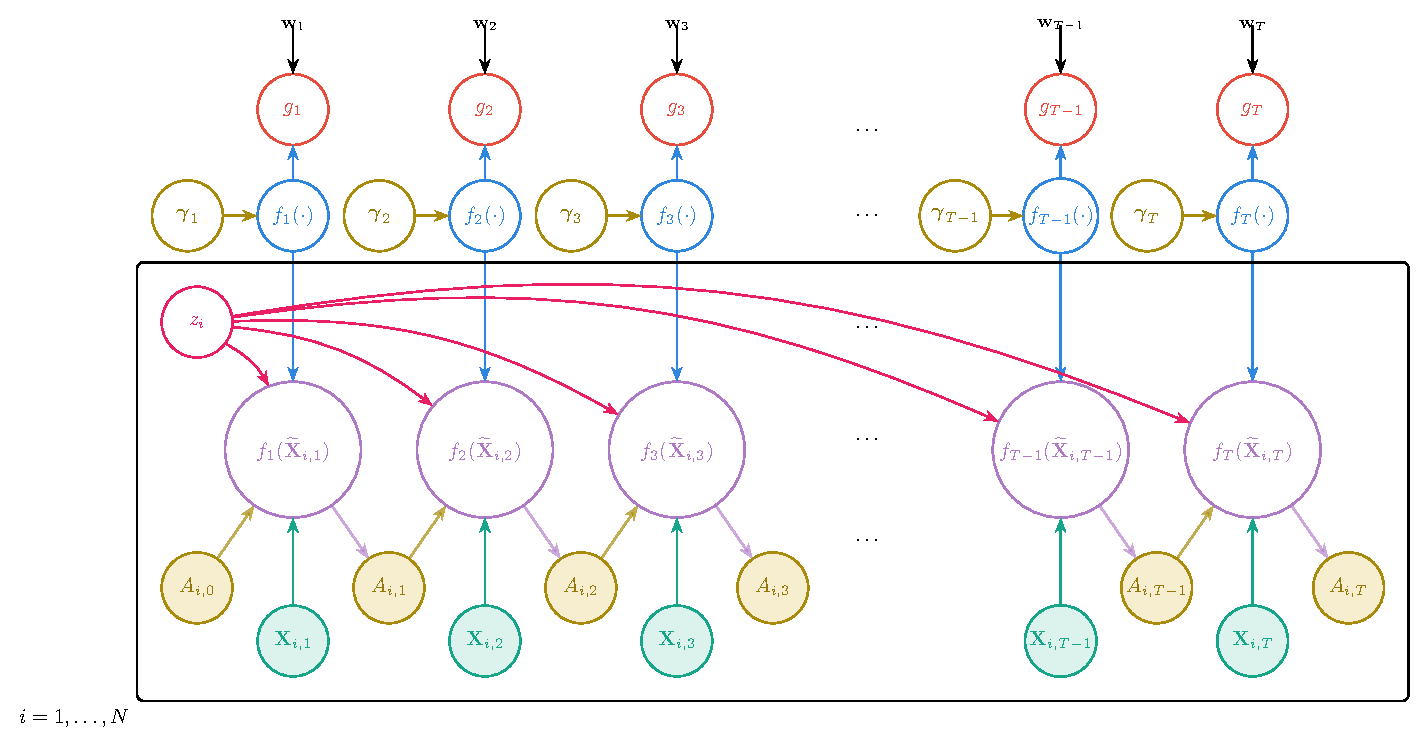
\includegraphics[width=\paperwidth,trim=0.5cm 0.5cm 0.5cm 0.5cm,
  clip]{figures/build/fit_seqgplvm_dag.pdf}
  \caption{Inference dag for the SeqGPLVM.}
  \label{fig:seqdecon-dag}
\end{figure}
\end{landscape}

\end{comment}


\chapter{Additional Simulation Results}
\label{sec:additional_simulation_results}
Figures~\ref{fig:simulation_bias_combined_a_p4}--\ref{fig:simulation_coverage_combined_a_p4} 
report the results of the simulation study for the four-covariate case. 
The additional results for the four-covariate case lead to the same overall conclusions as in 
the two-covariate setting. Figure~\ref{fig:simulation_bias_combined_a_p4} reports the bias, 
Figure~\ref{fig:simulation_standard_error_combined_a_p4} reports the standard error, and 
Figure~\ref{fig:simulation_coverage_combined_a_p4} reports the coverage. 
Within each figure, the first two rows correspond to the weak unmeasured confounding setting 
($c_U=1$), and the last two rows correspond to the strong unmeasured confounding setting 
($c_U=2$). The first and third rows correspond to $\tau_F=1$, while the second and fourth 
rows correspond to $\tau_C=0.3$. The columns correspond to the $N$ to $T$ ratio, with 
panels (A), (D), (G), and (J) showing $\rho=5$, panels (B), (E), (H), and (K) showing 
$\rho=10$, and panels (C), (F), (I), and (L) showing $\rho=50$. 
In particular, both \texttt{FE-MSM} and \texttt{SeqGPLVM-MSM} 
still improve over the naive \texttt{IPTW} estimator, while \texttt{FE-MSM} remains uniformly 
closer to \texttt{IPTW-True} and exhibits smaller estimated standard errors than \texttt{SeqGPLVM-MSM}. 
However, increasing the number of observed covariates from \(d_X=2\) to \(d_X=4\) does not lead to a systematic 
finite-sample improvement. Across scenarios, the \(d_X=4\) results are generally associated with larger average 
standard errors (Figure~\ref{fig:simulation_standard_error_combined_a_p4}). 
Although coverage occasionally improves in the more difficult settings, especially under stronger unmeasured 
confounding, these improvements appear to be driven mainly by wider intervals rather than smaller bias 
(Figures~\ref{fig:simulation_bias_combined_a_p4} and~\ref{fig:simulation_coverage_combined_a_p4}, panels (G)--(L)). 
As in the main results, the most challenging regime remains the short-panel setting with \(\rho=50\), 
particularly for smaller sample sizes, where the performance of both adjusted estimators deteriorates especially 
for \texttt{SeqGPLVM-MSM} (Figures~\ref{fig:simulation_bias_combined_a_p4}--\ref{fig:simulation_coverage_combined_a_p4}, panels (C), (F), (I), and (L)).
\begin{figure}[!tbp]
    \centering
    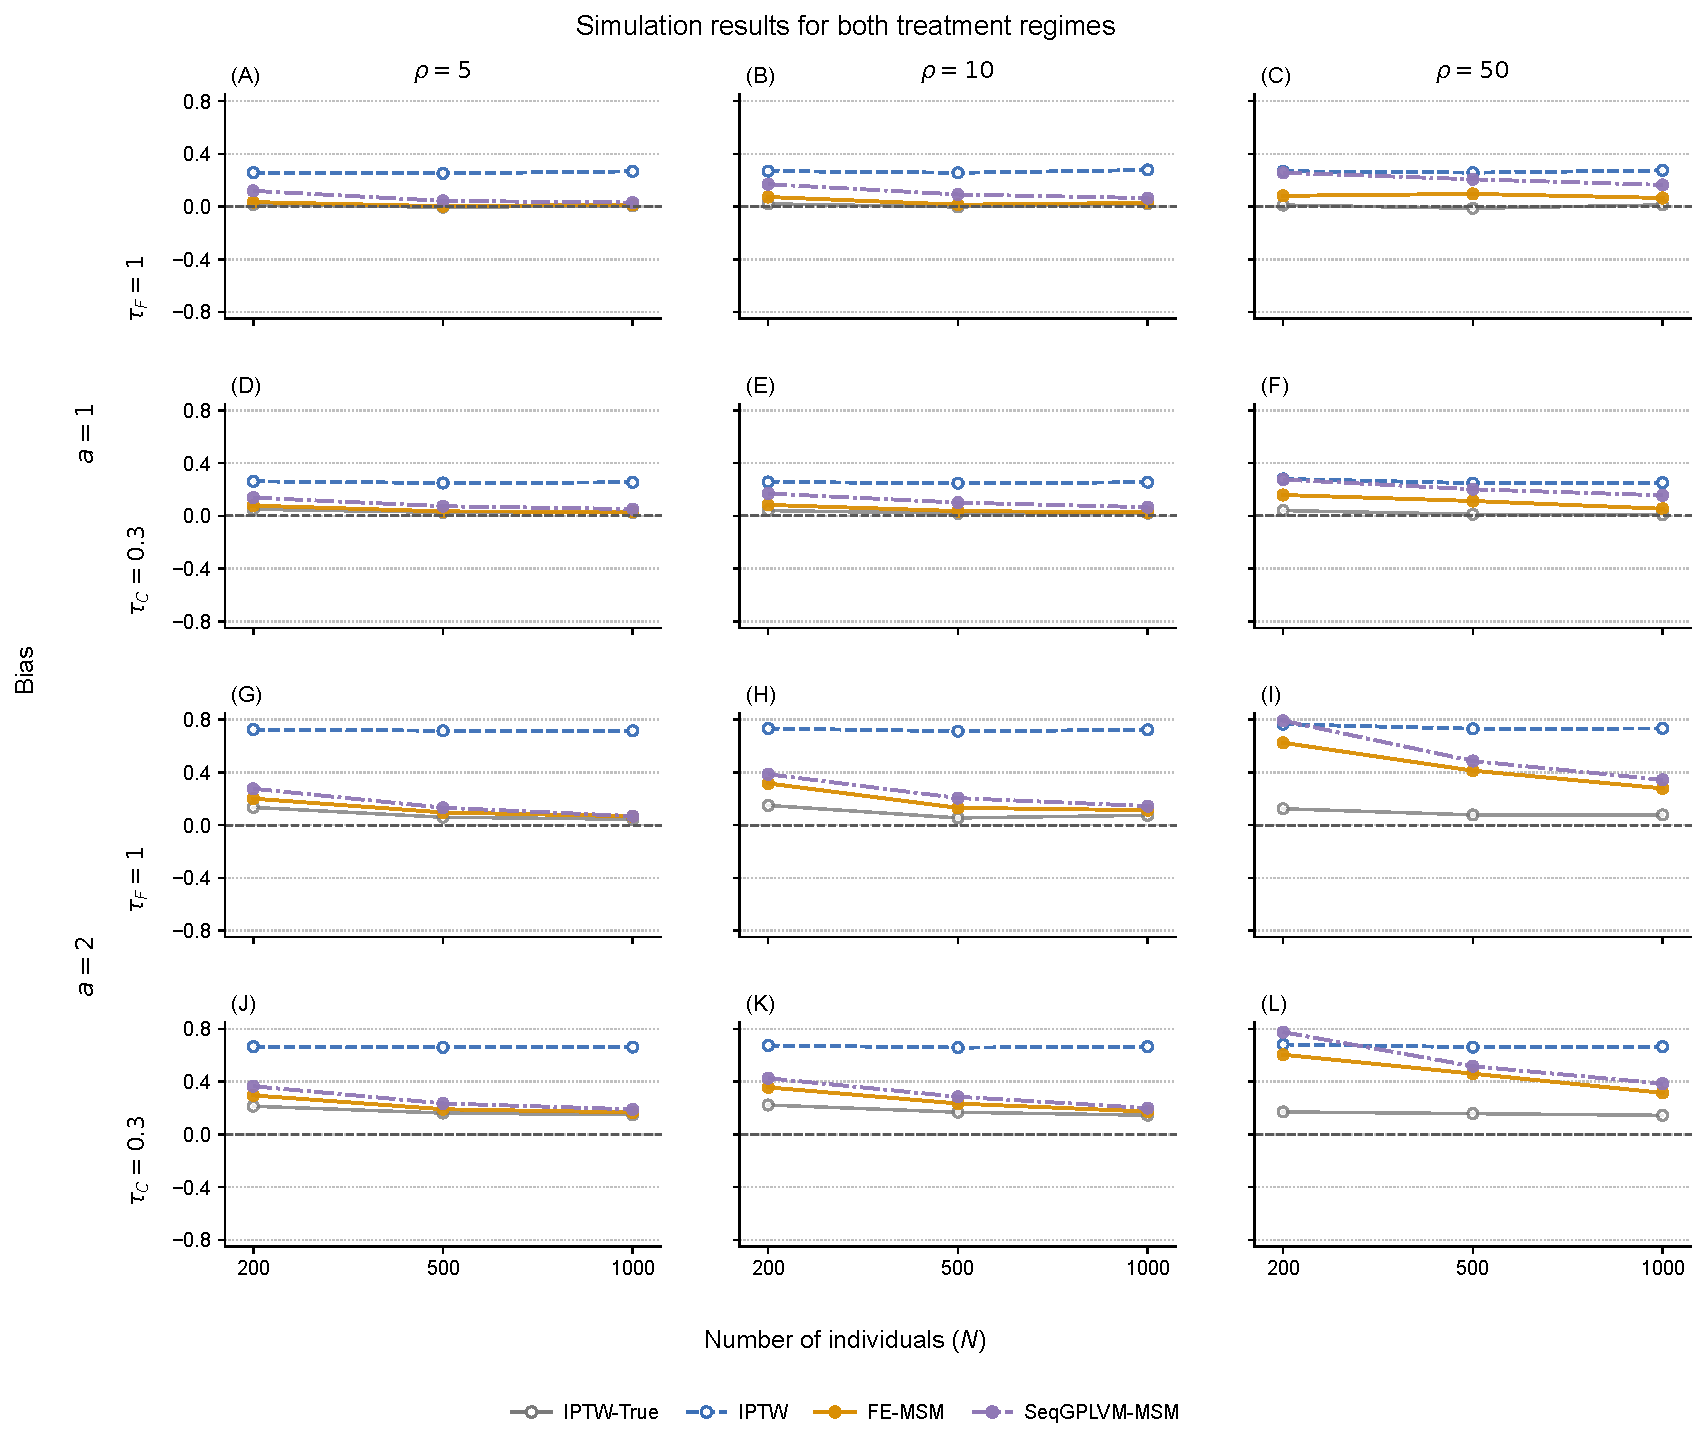
\includegraphics[width=\textwidth]{figures/build/simulation_bias_combined_a_p4.pdf}
    \caption{Simulation bias for the four-covariate case. The panels report bias for $c_U=1$ and $c_U=2$, for $\tau_F=1$ and $\tau_C=0.3$, across sample sizes $N$ and ratios $\rho = N/T$.}
    \label{fig:simulation_bias_combined_a_p4}
\end{figure}

\begin{figure}[!tbp]
    \centering
    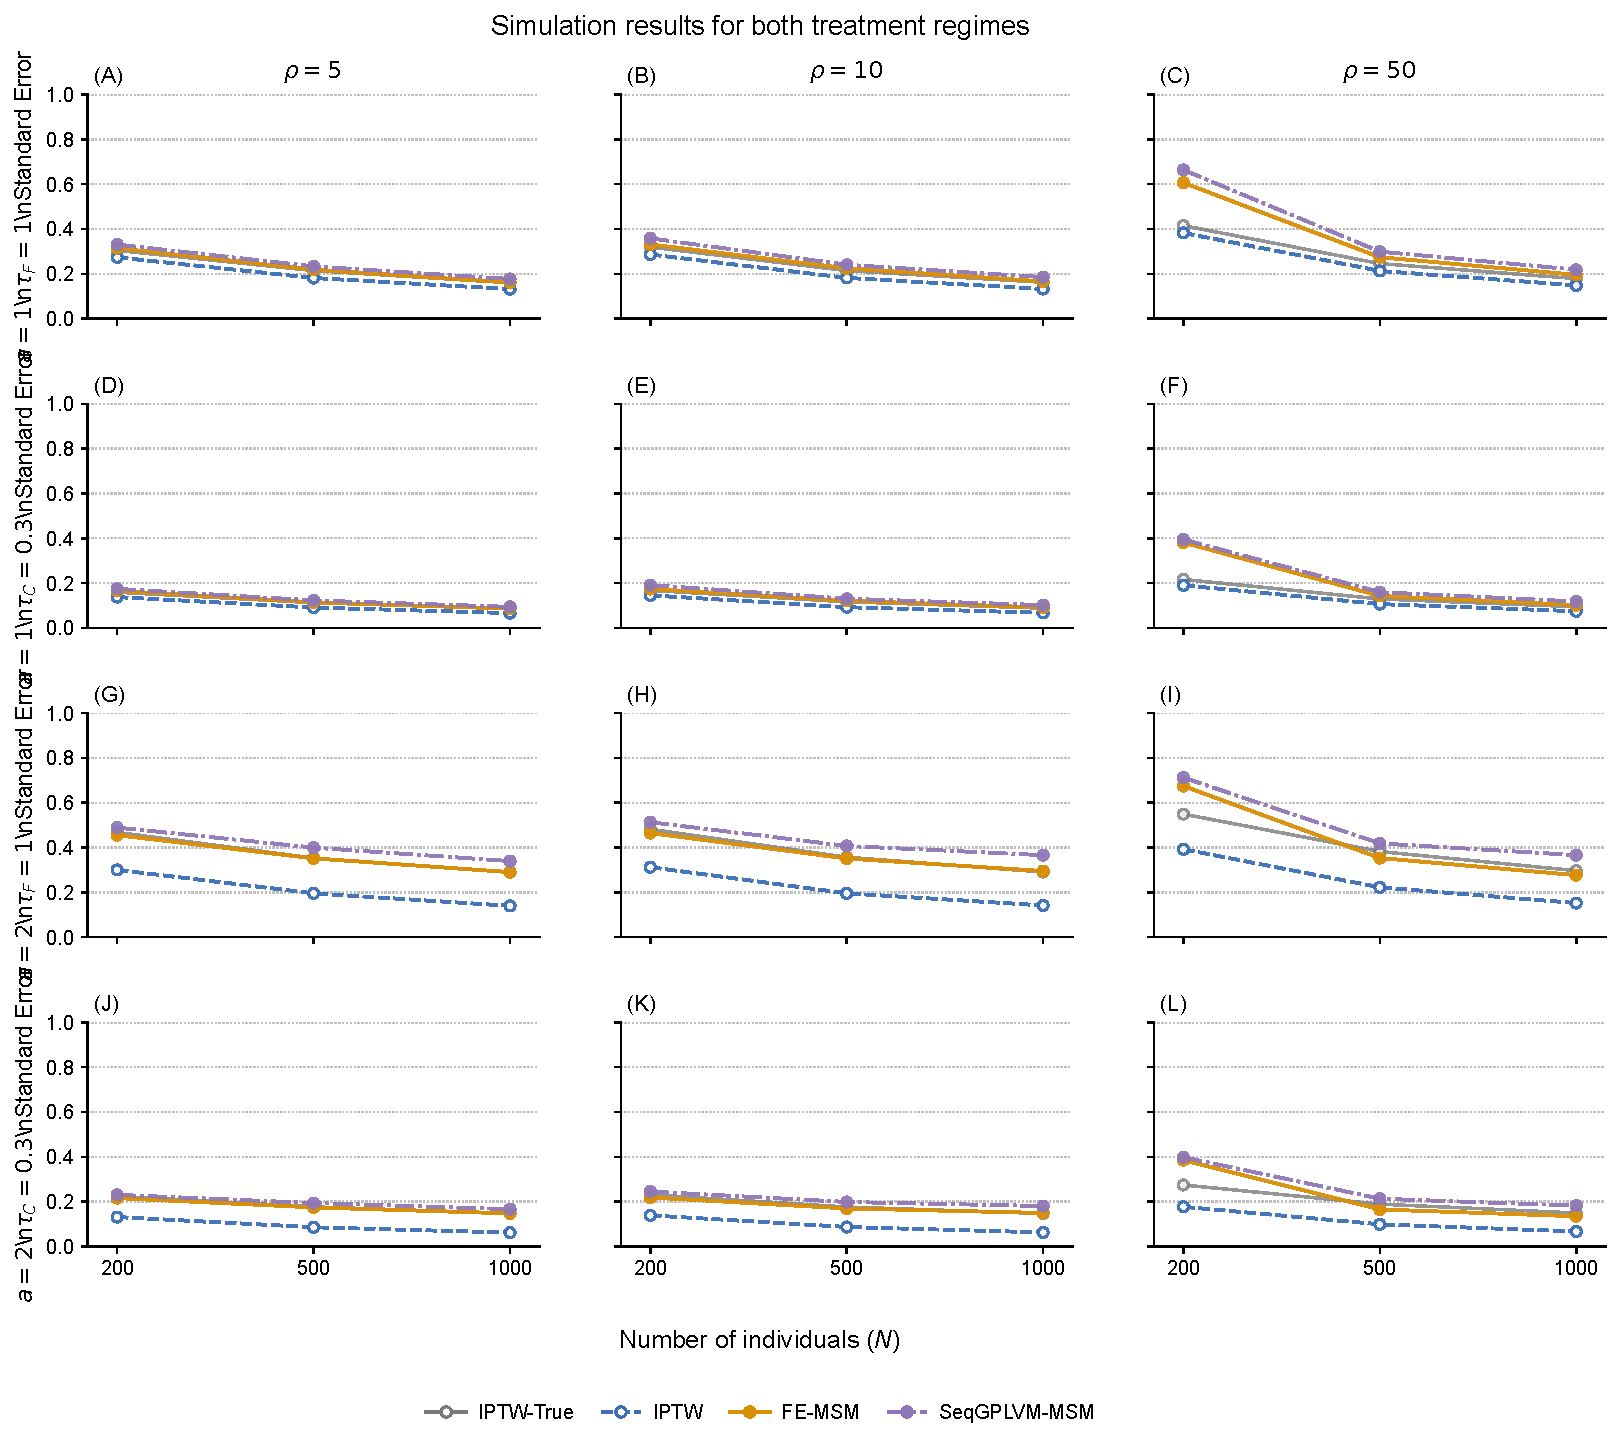
\includegraphics[width=\textwidth]{figures/build/simulation_standard_error_combined_a_p4.pdf}
    \caption{Simulation standard error for the four-covariate case. The panels report standard error for $c_U=1$ and $c_U=2$, for $\tau_F=1$ and $\tau_C=0.3$, across sample sizes $N$ and ratios $\rho = N/T$.}
    \label{fig:simulation_standard_error_combined_a_p4}
\end{figure}

\begin{figure}[!tbp]
    \centering
    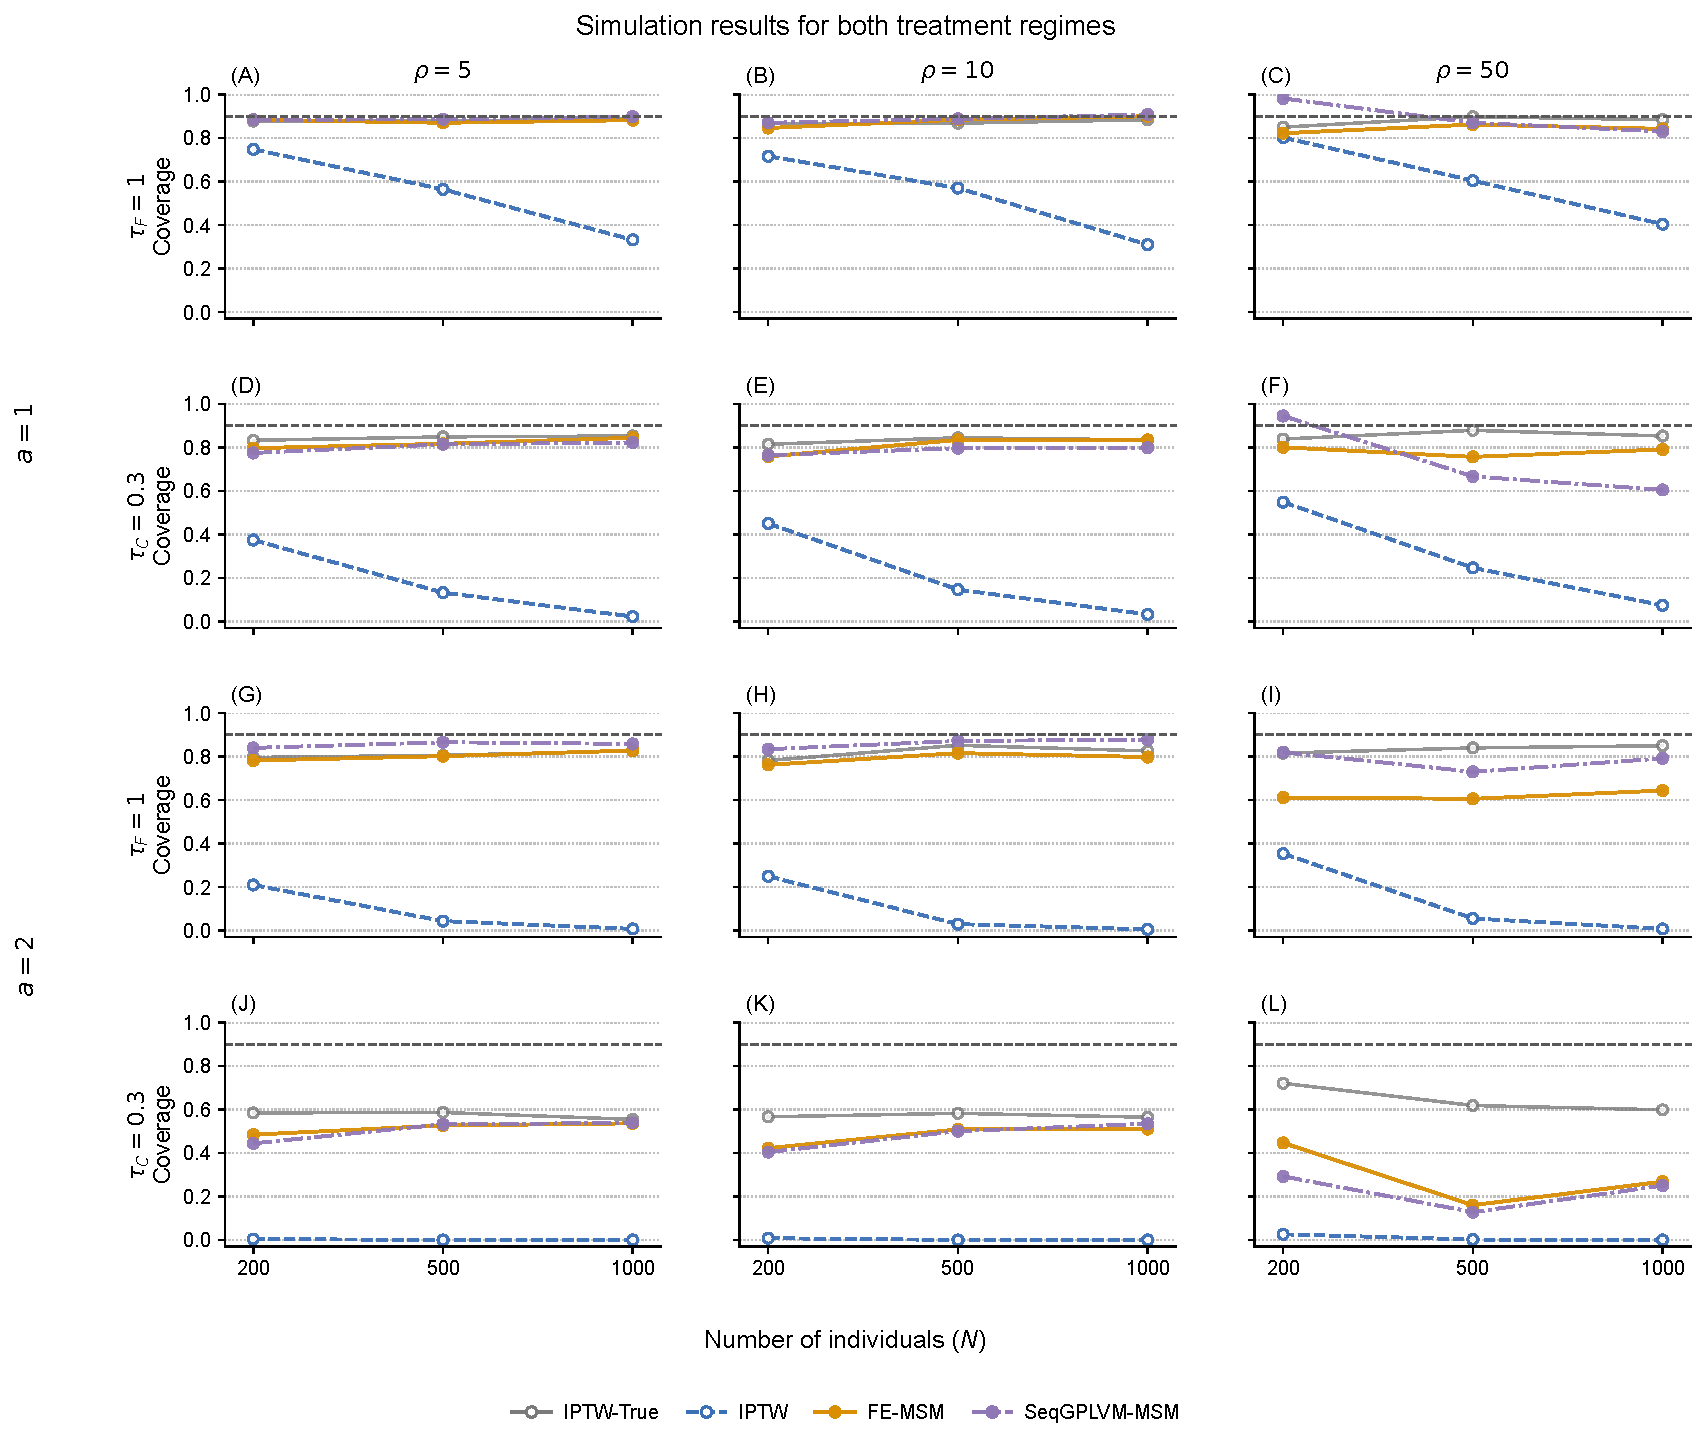
\includegraphics[width=\textwidth]{figures/build/simulation_coverage_combined_a_p4.pdf}
    \caption{Simulation coverage for the four-covariate case. The panels report coverage of the 90\% confidence intervals for $c_U=1$ and $c_U=2$, for $\tau_F=1$ and $\tau_C=0.3$, across sample sizes $N$ and ratios $\rho = N/T$.}
    \label{fig:simulation_coverage_combined_a_p4}
\end{figure}

%\input{sections/supplementary}

\end{document}